% !TEX root = ../These_Robin_Master.tex
\chapter{Évaluer un modèle de simulation complexe en situation d'inter-disciplinarité}
\begin{center}
{\large Version \hl{2018-12-18}}
\end{center}
\minitoc

\clearpage
\setlength{\epigraphwidth}{0.7\textwidth}
\epigraph{Although the construction and analysis of a simulation model, the validity of which has not been ascertained by empirical observation, may prove to be of interest for expository or pedagogical purposes (e.g., to illustrate particular simulation techniques), such	a model contributes nothing to the understanding of the system being simulated.
[...]\\
Unless the construction of simulation models is viewed as a game with no purpose other than the formulation of a model, it is hard to escape the conclusion that the purpose of a simulation experiment is to predict some aspect of reality.
}{\cite[B-92-93;96]{naylor_verification_1967}}


\section{Comment évaluer un modèle ?}

Depuis les travaux précurseurs en simulation informatique \autocite{naylor_verification_1967,hermann_validation_1967,sargent_validation_1979} jusqu'aux recherches contemporaines \autocite{amblard_evaluation_2006,banos_pour_2013,augusiak_merging_2014, rey-coyrehourcq_plateforme_2015}, la plupart des chercheurs ont toujours mis en avant qu'un modèle de simulation non évalué n'avait ni utilité (pour les plus anciens), ni validité.
Sans caricaturer ces écrits, on peut noter que tous cantonnent les modèles non évalués à des \og jeux\fg{} ou encore, pour les plus modérés, à des outils uniquement pédagogiques.

Comme indiqué dans le chapitre 1 (\hl{REF}), nous inscrivons SimFeodal comme un modèle résolument pédagogique, et l'on pourrait dès lors se passer d'en mener une évaluation quelconque.
Il nous semble pour autant que l'exercice intellectuel que constitue la (co-)construction d'un modèle de simulation perdrait de son intérêt intrinsèque s'il ne donnait lieu à des procédures, quelles qu'elles soient, ayant pour objectif de d'en assurer une certaine qualité, à défaut d'en garantir une validation stricte.

Nous sommes en effet convaincu que même pour des modèles visant à \og assister la construction de théories\fg{}\footnote{ \og [...] Simulation models to support theory building -- so-called heuristic modelling -- [...].\fg{}} pour reprendre les termes de \cite[260]{lake_trends_2014}, ou encore, selon la classification alternative de l'auteur, pour les modèles à usage \og de développement\fg{}\footnote{\og 'developmental' utility\fg{}, c'est-à-dire les modèles dont le développement et l'implémentation bénéficient aux chercheurs qui y prennent part plutôt qu'à ceux qui se contentent de les utiliser a posteriori.}, les différents outils d'évaluation permettent d'acquérir une connaissance précieuse sur l'objet modélisé, ne serait-ce que par les effets collatéraux qu'entraîne l'évaluation d'un modèle.
Soit-il à visée pédagogique, à base d'agents, de type descriptif ou encore vu comme \og hybride\fg{}, un modèle de simulation demeure un modèle qu'il convient d'évaluer pour être en mesure d'en tirer des connaissances \autocite[299-300]{sargent_history_2017}.

Sans entrer dans les spécificités conceptuelles de ce qu'est l'évaluation de modèle ou de l'histoire de ces méthodes\footnote{En particulier parce que ce sujet a été très largement traité dans un travail de thèse récent au sein de notre laboratoire de recherche \autocite[pp. 58--184]{rey-coyrehourcq_plateforme_2015}, travail auquel nous renvoyons vivement pour plus d'approfondissements.}, nous nous contenterons dans la suite de cette partie de donner une vision aussi succincte que possible de ce qu'est l'évaluation, en particulier pour en dégager les méthodes employées usuellement.
Cela nous permettra en particulier de défendre et de promouvoir l'une de ces méthode, la validation visuelle, que nous jugeons très adaptée dans le cadre de co-constructions interdisciplinaires de modèles.

\subsection{Évaluation, validation, vérification\ldots : désambiguïsation}

Il nous semble important de commencer cette partie par un point de définition et de clarification des concepts mobilisés, non pas par convention datée, mais parce que les usages en matière d'emploi des termes d'évaluation, de validation (méthodologique, formelle\ldots) ou encore de vérification sont particulièrement diffus et trompeurs dans la littérature relative à la modélisation, y compris dans le champ plus restreint de la simulation à base d'agents en sciences humaines et sociales.

Depuis les travaux fondateurs, dans les années 1960, la logique qui consiste à éprouver un modèle -- c'est-à-dire à vérifier qu'il corresponde correctement d'une part au système qu'il décrit, et d'autre part à la manière dont il est décrit -- donne lieu à différentes terminologies.
On notera en particulier que les deux articles considérés comme pionniers, tous deux parus en 1967, reposent pour l'un sur la notion de vérification \autocite{naylor_verification_1967}, et pour l'autre sur celle de validation \autocite{hermann_validation_1967}, sans pour autant que la distinction entre les deux approches puisse être vue comme consistante.
Quelques décennies plus tard, une fois la pratique de simulation informatique plus développée et mûre, un consensus de pratique a été adopté autour de l'expression englobante de "Validation, Verification and Testing techniques (VV\&T)", par l'entremise d'une proposition d'Osman Balci \autocite{balci_validation_1994} de clarification et de définition de chacun de ces composants.
Pour reprendre ses mots en une distinction devenue courante en simulation à base d'agent, la \textit{validation} consiste à concevoir le bon modèle\footnote{\og Model validation deals with building the \textit{right} model.\fg{}} alors que la \textit{vérification} permet de s'assurer que le modèle est bien construit\footnote{\og Model verification deals with building the model \textit{right}.\fg{}}.
Le \og \textit{Testing}\fg{} correspond aux techniques mises en œuvre, et s'applique donc indistinctement à ces deux composantes.

En dépit de cette définition stricte, les usages persistent à ne pas formellement différencier vérification et validation, le plus souvent en englobant ces pratiques dans le terme plus large et moins défini d'\og évaluation\fg{}.
Il n'est d'ailleurs pas rare que ces trois termes soient employés de manière interchangeable, voir intervertie, comme un recensement rigoureux des usages le démontre \autocite[Table 1, p. 120]{augusiak_merging_2014}.

\paragraph*{}
Nous partageons le besoin formel -- identifié par les auteurs de cette étude~-- de définir un nouveau terme -- \og \textit{evaludation} \fg{} dans leur proposition~-- et nous souscrivons à leur approche de définition (\cref{fig:schema_evaludationl}).
Nous nous contenterons toutefois, dans ce travail, de nous inscrire dans les choix de \cite{amblard_evaluation_2006}, en particulier parce qu'ils nous semblent assez largement adoptés dans la communauté scientifique de modélisation en sciences humaines et sociales francophone.
Pour ces auteurs, et donc dans le présent ouvrage, on emploie le concept d'\textbf{évaluation} pour définir l'approche d'ensemble, et on distingue alors \og \textbf{validation interne}\fg{} -- correspondant à la \textit{verification} définie par Balci, c'est-à-dire s'assurer de la bonne conception du modèle, et \og \textbf{validation externe}\fg{} -- ce que Balci nomme \textit{validation}, soit l'assurance que le modèle est adapté à ce qu'il cherche à représenter.


\begin{figure}[H]
	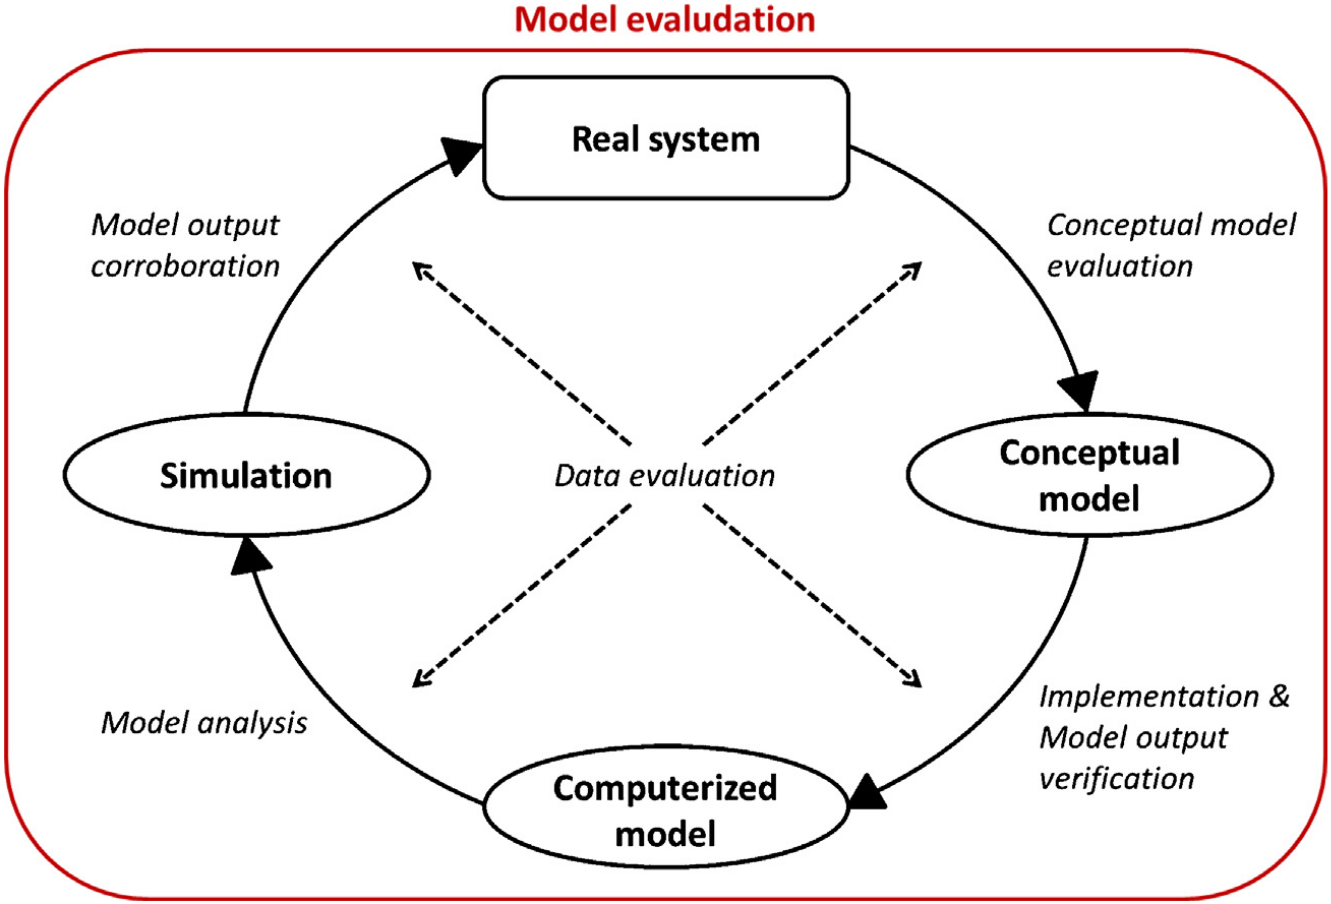
\includegraphics[width=\linewidth]{img/Schema_Augusiak_evaludation.png}
	\caption{Représentation schématique du cycle de modélisation et de la typologie des termes relatifs à l'évaluation de modèle, dans \cite[Fig. 1, p. 121]{augusiak_merging_2014}}
	\label{fig:schema_evaludationl}
\end{figure}

\begin{quotation}
\og Il est classique de différencier deux étapes dans la validation : interne et externe.
\begin{itemize}
	\item La phase de vérification ou \textbf{validation interne} comprend d'abord une vérification de conformité entre les spécifications et le programme implémenté et pose la question : est-ce que le modèle implémenté est bien celui que je voulais implémenter ? [...]
	Ensuite, la validation interne concerne la recherche et l'identification des propriétés du modèle.
	Dans le cas des simulations multi-agents, des preuves logiques ne peuvent être obtenues et se pose alors la question : est-ce que mon modèle possède les propriétés attendues ?
	Parmi ces bonnes propriétés, on considère par exemple la robustesse ou des études de sensibilité pour vérifier si les réponses sont bien différenciées sur l'espace des paramètres.
	Cette phase de validation interne concerne de fait une validation dans le contexte ou la logique propre du modèle.

	\item La deuxième phase de validation, la \textbf{validation externe}, correspond à l’évaluation de l’adéquation entre le modèle et le phénomène réel dont il est censé rendre compte.
	Pour cette dernière phase, la comparaison aux données empiriques ou le fait que le modèle soit capable d'exhiber des faits stylisés identifiés sur le système modélisé sont des critères clés.
\end{itemize}
Ainsi, ce qui est étudié au travers des simulations, ce sont tout d’abord les propriétés systémiques (structurelles et dynamiques) du modèle, les formes qui peuvent apparaître du fait des hypothèses posées (validation interne) ; ensuite est évaluée la pertinence du modèle vis-à-vis de situations que l’on souhaite représenter ou prévoir (validation externe).\fg{}\\
	\mbox{}~ \hfill \cite[110-111]{amblard_evaluation_2006}
\end{quotation}


\clearpage

\subsection{Les étapes de l'évaluation de modèle}


\clearpage
+ Mettre schéma des phases (selon \autocite{hermann_validation_1967} vs  \autocite{naylor_verification_1967} ? Ou \autocite{klugl_validation_2008}?) + Mentionner \cite{sargent2009verification} + Finir sur \cite{amblard_assessment_2007} : validation interne/externe etc.


\subsection{\og Face validity\fg{} dans l'approche classique}



\begin{quotation}
	\og Face validity is a surface or initial impression of a simulation or game's realism.

	Probably no approach to model validity is reported more frequently than the subjective estimates of experimenters, observers, or human participants as to the correspondence between the model's operation and their perception of the actual phenomena which the game or simulation represent.

	[...]

	Face validity can be a significant part of a validity strategy. A quick impression that "things don't seem right" may be the only validity check possible during the actual operation of a game or simulation. Such validity judgments and their evaluation may also be part of the learning experience provided by operating models designed for instructional purposes.

	[...]

	Although face validity has value in the early stages of model building or for quick checks during actual operation, its severe limitations should be recognized. Sometimes the experimenter will not know what behaviors are "realistic" because of his limited experience observing the actual phenomena. Participants can become interested and highly motivated in an incorrect representation of the desired environment. If the simulation involves the substitution of one property for another, some features may appear quite unreal and yet replicate the performance of the reference system for which the simulation was designed. The acceptance of face validity as a rough, first approximation might be improved if the simulator explicitly stated in advance what observations would constitute indications that an aspect of the observable universe had been successfully captured. In summary, face validity in its usual form suffers from the lack of explicit validity criteria.\fg{}\\
	\mbox{}~ \hfill \cite[221-222]{hermann_validation_1967}
\end{quotation}


\begin{figure}[H]
	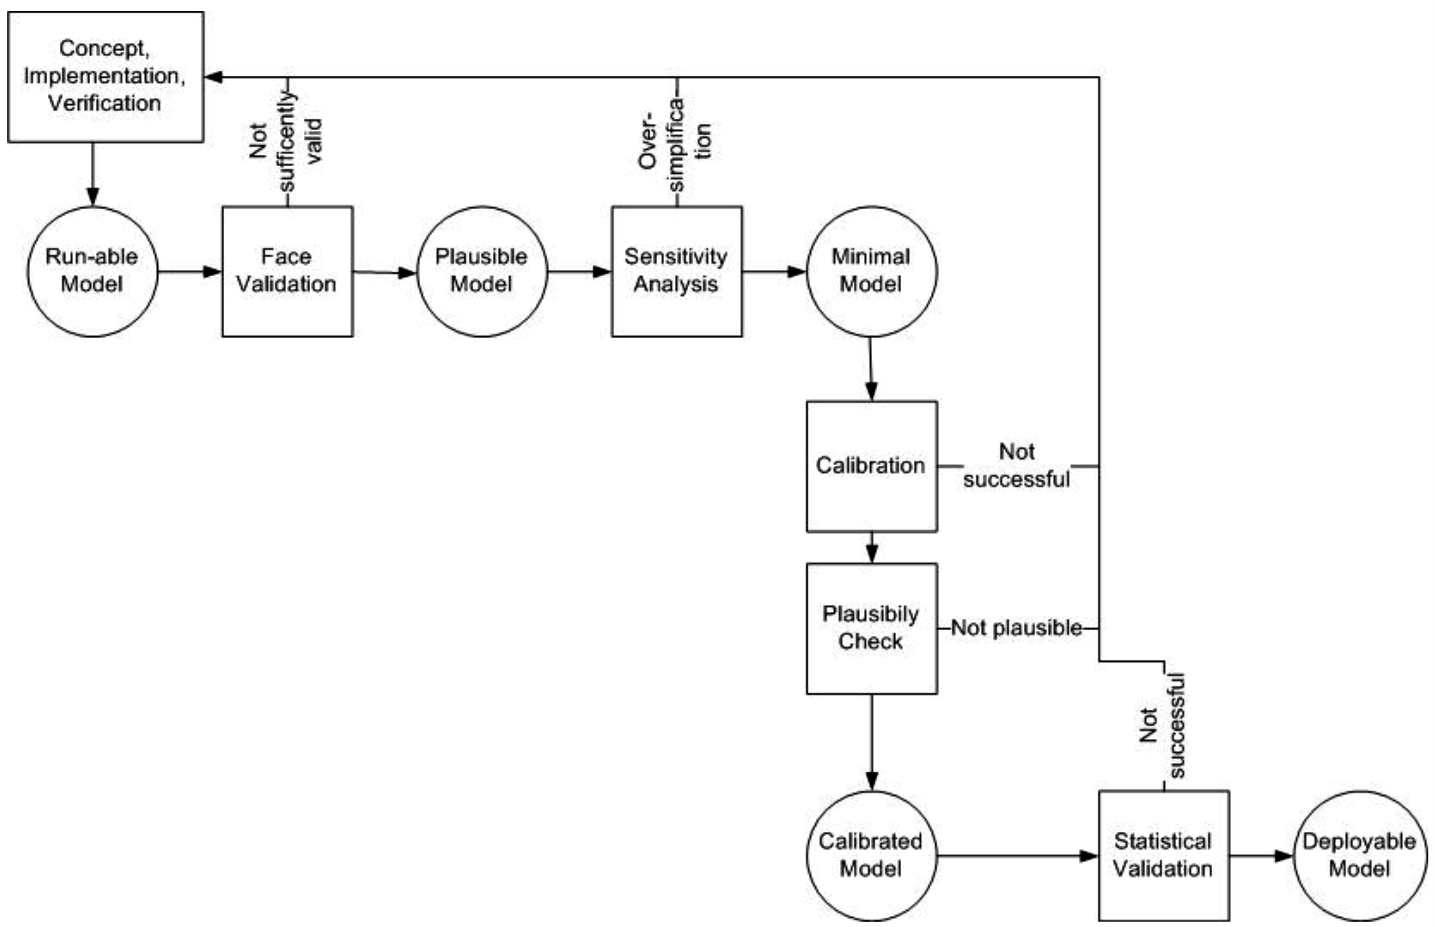
\includegraphics[width=\linewidth]{img/Schema_Kluegl.png}
	\caption{\og Sketch of a general procedure for validating an agent-based simulation\fg{}, \cite[fig. 1 p. 42]{klugl_validation_2008}}
	\label{fig:schema_kluegl}
\end{figure}

\begin{figure}[H]
	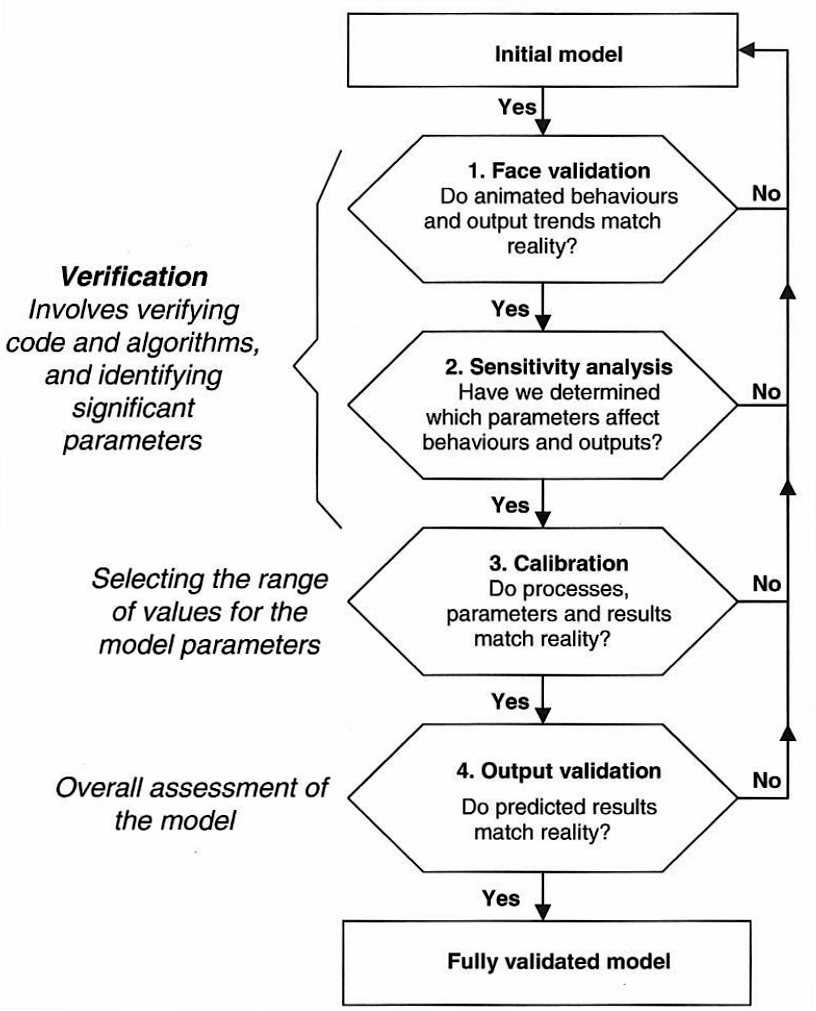
\includegraphics[width=.6\linewidth]{img/Schema_Ngo.png}
	\caption{\og General validation process of an ABM\fg{}, \cite[fig. 10.1 p. 183]{ngo_calibration_2012}}
	\label{fig:schema_ngo}
\end{figure}


\begin{quotation}
\og Face validity can be seen as the result of face validation. Under this paradigm I want to subsume all methods that rely on natural human intelligence. Examples are structured walk-through, expert assessments of descriptions, animations or results. Thus, face validity shows that processes and outcomes are reasonable and plausible within the frame of theoretic basis and implicit knowledge of system experts or stake-holder. Face validation may be applied from the early phases of the simulation study under the umbrella of conceptual validations. It is often also called plausibility checking.

[...]

One may argue why face validity is need, when statistical validation is successfully done? Face validation assures that the processes and structures are reasonable for a human expert. Especially, when there is (semi-)automatic calibration of a simulation that is used in combination with statistical validation, a careful check of plausibly is necessary. This is in general true for all kinds of simulation, but it is particularly important for agent-based simulations.\fg{}\\
\mbox{}~ \hfill \cite[39-40]{klugl_validation_2008}
	\end{quotation}

\begin{quotation}
\og Face validation usually plays an important role during
model design. All tests based on reviews, audits, involv-
ing presentation and justification of assumptions and model
structure are used for reaching this form of plausibility. Face
validation in this phase of model development consists of at
least three methodological elements executed by potentially
different human experts :
\begin{itemize}
	\item \textbf{Animation Assessment} A human expert assesses the animation of the overall simulated system (or of parts of it) whether the simulated system appears to behave like the original system. [...]
	\item \textbf{Output Assessment} Simulation output can also be assessed by a human expert checking the plausibility of the absolute values, relations between different values and also the dynamics and trends of the different output values of simulation runs. It can be applied on the macro as well as on the agent level. If intended relations can be formalized, e.g. in forms of constraints, output assessment can be automatized.
	\item \textbf{Immersive Assessment} A human expert looks through the eyes of one particular agent and sees what the agent perceives and how it reacts on it. Based on this information the human can evaluate directly whether the behavior of the simulated agent is appropriate. If the interface allows participation, the human may also assess the behavior of the other agents in reaction to interactions with the human-controlled agent. Clearly, the success of these tests depends on the appropriateness of the interface which may even be particular for every agent.
\end{itemize}
The question that remains here is about the best order to apply the different tests. I suggest to start with the animation and immersion tests and only when they are passed the output testing should be applied. The reason for this is simply the assumption that runs of an agent-based simulation are expensive and have to be repeated several times due to stochasticity. It is comparatively cheap to have a look onto animation. Thus, one should start with cheap tests that allow fast rejection of the model and continue investing more and more effort when the model becomes more and more valid.\fg{}
\mbox{}~ \hfill \cite[41-42]{klugl_validation_2008}
\end{quotation}


\begin{quotation}
\og Although face validation may be informal and inconsistent, but it at least results in plausibility of modeled processes. Our experience with modeling and simulation in many interdisciplinary projects showed that even the formulation of a plausible model supports theory building and future empirical research.\fg{}
\mbox{}~ \hfill \cite[43]{klugl_validation_2008}
\end{quotation}





Différencier Face validity (vraisemblance) et visual validation

\subsection{Vers une validation visuelle}

\cite[Table 3, p. 46]{balci1998verification} : Face validity applicable à toutes les étapes du cycle de vie de la simulation

\begin{quotation}
		\textbf{Informal methods} [...]\\
		\og Face validation is a validation method that compares simuland behavior to model results. In face validation, observers who may be potential  users  of  the  model  and/or  subject  matter  experts  with  respect  to  the  simuland  review  or  observe  the  results  of  a  simulation  (an  execution  of  the   executable model). Based on their knowledge of the simuland, the observers  subjectively compare the behavior of the simuland as refl ected in the simulation results with their knowledge of the behavior of the actual simuland under the  same  conditions,  and  judge  whether  the  former  is  acceptably  accurate. Differences  between  the  simulation  results  and  the  experts' expectations may indicate model accuracy issues.

		[...]

		While  face  validation  is  arguably  most  appropriate  for  such  interactive simulations, it is often used as a validation method of last resort, when a shortage of time or a lack of reliable data describing simuland behavior precludes the  use  of  more  objective  and  quantitative  methods.  While  moving  beyond face validation to more objective and quantitative methods should always be a goal, face validation is clearly preferable to no validation at all.\fg{}\\
	\mbox{}~ \hfill \cite[341-342;]{petty2010verification}
\end{quotation}




\subsection{Des critères pour la validation : les indicateurs}

\subsection{L'importance de la réplication}

\clearpage
\section{Évaluer le modèle SimFeodal}

Le modèle SimFeodal présenté dans le chapitre 2 correspond à une « version 0 » du modèle souhaité, c'est-à-dire qu'il en constitue une première pré-version.
	L'ensemble des mécanismes figurant dans le modèle conceptuel ont été implémentés mais l'ensemble des liens, interactions et valeurs de paramètres ne sont pas encore stabilisés.
	De ce fait les résultats des simulations ne répondent pas nécessairement aux attentes définies au \hl{§XX}.
	Si l'on a déjà décrit le principal objectif du modèle dans le chapitre précédent (celui de comprendre les mécanismes sous-jacents au processus de polarisation qui s'est déroulé entre 800 et 1100), il convient ici d'expliciter comment les résultats d'un tel processus peuvent être saisis.
Ceux-ci sont en effet nombreux et hétérogènes, concernant aussi bien des concentrations de foyers paysans que l'émergence de pôles.
Certains sont centraux, d'autres secondaires, et le modélisateur a des attentes relativement à l'ensemble des résultats obtenus en fin de simulation.
La description précise de ces attentes se révèle importante dans le cadre du paramétrage -- et de l'ensemble des étapes de la vie du modèle -- de SimFeodal.
Dans cette partie, on explicitera d'abord le sens que l'on prête à ces attentes, sous la forme « d'indices empiriques » et « d'indicateurs de sortie de simulation ».
Ces indices et indicateurs sont nombreux, certains sont multivariés, et il s'agira donc de présenter des méthodes visant à réduire la complexité de ces indicateurs de sortie, en adoptant une démarche proche de ce qui se fait en statistiques : réduction de dimensionnalité et/ou catégorisation et hiérarchisation de ces indicateurs.
En mobilisant ces méthodes, on pourra ensuite décrire et qualifier le comportement du modèle SimFeodal tel qu'il a été décrit, dans sa « version 0 », dans le chapitre précédent (\hl{ref}).

\subsection{Indices et indicateurs}

On attend d'un modèle, sans entrer encore dans le détail, qu'il reproduise au moins les grands traits de l'élément empirique dont il cherche à rendre compte.
Ces grands traits peuvent s'entendre de multiples manières, et se formaliser avec encore plus d'approches.
Ici, nous avons souhaité proposer une dichotomie simple entre le domaine de l'empirique et celui de la simulation, en systématisant l'usage d'un vocabulaire qui est souvent employé de manière plurielle.
Pour être en mesure d'évaluer la vraisemblance du comportement reproduit par le modèle sur le plan empirique, il est nécessaire de mettre en correspondance des éléments empiriques et des éléments issus de la simulation.
Nous caractérisons ces éléments en deux grands ensembles :
(1) \textbf{les indices empiriques}, éléments quantifiables ou au moins descriptibles émanant du domaine empirique, et  (2) \textbf{les indicateurs de sortie}, variables informatiques produites par le modèle de simulation et devant pouvoir être comparés à chacun des indices empiriques.
La \cref{fig:schema_indices} reprend, sous forme de schéma ontologique synthétique, ces deux ensembles de mesures, explicitant le vocabulaire mobilisé dans cette partie.

\begin{figure}[H]
\captionsetup{width=\linewidth}
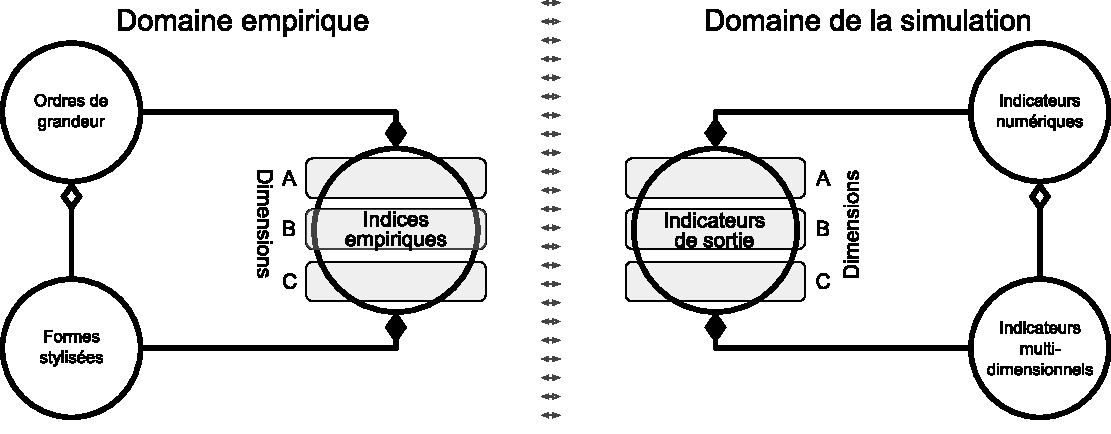
\includegraphics[width=\linewidth]{img/schema_indice_indicateur.pdf}
\caption{Schéma de synthèse des correspondances entre mesures relevant du domaine empirique et mesures issues des simulations pour l'évaluation du modèle SimFeodal.\\
\todobox{Lena : Paragraphe difficile}
La correspondance des éléments est représentée par une symétrie axiale, entre d'un côté des \og indices empiriques\fg{} et de l'autre des \og indicateurs de sortie de simulation\fg{}.
Les losanges pleins désignent une relation de composition :
un \og indice empirique\fg{} est soit un ordre de grandeur, soit une forme stylisée.
Les losanges vides indiquent une relation d'agrégation :
une forme stylisée est une agrégation d'ordres de grandeurs.
Les dimensions (A à C) regroupent des indices (et les indicateurs qui leur correspondent) qui peuvent être de plusieurs types, et sont elles aussi comparables et en correspondance entre les domaines.
}
\label{fig:schema_indices}
\end{figure}


\subsubsection{Les indices empiriques}

Afin d’évaluer la capacité du modèle à reproduire un phénomène observé, il est nécessaire de disposer dans le domaine empirique, de \og points de repère\fg{}.
Selon les modèles, ceux-ci peuvent revêtir de multiples formes et relever de l'ensemble des échelles spatiales et temporelles que l'on choisit de mettre en scène dans le modèle.
Leur point commun est qu'ils doivent pouvoir être mesurés, au sens le plus large, c'est-à-dire être en capacité d'être reproduits et comparables avec d'autres mesures.
Dans cette étude, on a décidé de qualifier ces points de repère d'\og\textbf{indices empiriques}\fg{} et de les regrouper en deux catégories basées sur la précision avec laquelle ils peuvent être décrits\footnote{\todobox{Lena : pas compris la note}\\Et non sur la précision de leur connaissance, cf. \cref{sssec:incertitude}}.
La \cref{fig:schema_indices} illustre cette catégorisation entre la première catégorie -- les ordres de grandeur -- et la seconde -- les formes stylisées --.

\paragraph{Ordres de grandeur}
La première catégorie est constituée d'\textbf{ordres de grandeurs} empiriques estimés -- avec une précision plus ou moins importante (\hl{cf. tableau 3 p. 317 du chap. TMD, à reproduire dans chap 2}).
Certaines valeurs empiriques sont ainsi connues, que ce soit d'après des sources primaires ou secondaires, et peuvent ainsi constituer des indices.
Par exemple, on connaît avec quasi-certitude le nombre d'églises paroissiales de la région Touraine en 1100.
D'autres valeurs empiriques sont en revanche issues d'estimations.
Tel est le cas, par exemple, du taux de foyers paysans isolés en fin de période.
Celui-ci ne peut être renseigné par des sources primaires et il a donc été nécessaire de l'estimer à partir de sources secondaires et en menant des extrapolations.
Il est cependant possible de construire des indicateurs de sortie de simulation offrant une correspondance presque exacte de ces différents indices observés ou estimés (cf. \ref{para:correspondance}, \cnameref{para:correspondance}, p. \pageref{para:correspondance}).
Il est dès lors possible de mener une comparaison entre données observées/estimées et données simulées.
Ces ordres de grandeur peuvent ainsi participer à l'évaluation du comportement du modèle simulé.

\paragraph{Faits et formes stylisés}
La seconde catégorie d'indice empirique est moins précise et ne repose pas sur une valeur observable ou estimable, mais plutôt sur la connaissance experte d'un phénomène.
Il s'agit des \og \textbf{faits stylisés}\fg{}\footnotemark{}, rendant davantage compte d'une tendance dans la forme d'une relation ou d'une organisation que les indicateurs.
On fait un large usage de ces faits stylisés en économie, mais aussi en géographie, par exemple quand on qualifie la tendance des systèmes de peuplement à se hiérarchiser.
La valeur de la pente associée à la courbe rang-taille d'un système de villes tend ainsi vers $1$ (\hl{Trouver ref, sans doute Pumain/Saint-Julien}) à mesure que le système évolue et se hiérarchise.
De la même manière, le modèle de transition démographique d'Adolphe Landry est un fait stylisé, énoncé à partir de l'observation de nombreuses récurrences de l'évolution des populations d'un pays en fonction de leurs taux de natalité et de mortalité.
Ces exemples montrent qu'au sein des faits stylisés, il y a une certaine diversité quant à la précision de leurs énoncés :
on peut quantifier précisément la courbe d'une relation rang-taille et l'allure de son évolution dans le temps, \toChange{alors que la courbe logistique}{phrase à reprendre} de la transition démographique nécessite davantage de mesures et est moins précise dans les paramètres de son énoncé.
Dans notre cas d'étude, les faits stylisés sur lesquels on s'appuiera seront des d'une part des \og allures\fg{} de courbes (par exemple l'évolution dans le temps d'un indicateur), d'autre part des formes de répartition spatiale, et enfin des \og allures\fg{} de courbes résultant d'une composition d'ordres de grandeurs.
Nous qualifierons le premier type de \og \textbf{formes stylisées} temporelles\fg{} (courbe logistique estimée pour la polarisation des foyers paysans par exemple), le second type de \og \textbf{formes stylisées} spatiales\fg{} (changement dans la forme d'occupation de l'espace par les agrégats entre le début et la fin de la période par exemple).


Le troisième type, \og \textbf{forme stylisée} organisationelle \fg{}, correspond à une forme repérable dans l'agrégation à l'échelle du système, comme dans l'observation des hiérarchies grâce aux courbes rang-tailles.
Notons que ces formes stylisées relèvent le plus souvent d'une agrégation ou d'une composition d'ordres de grandeurs (comme figuré dans la \cref{fig:schema_indices}) :
l'évolution dans le temps de la population, par exemple, correspond à un vecteur d'ordres de grandeur, c'est-à-dire à une succession de mesures de la quantité de population pour chaque date étudiée.
\Lena{Même dans le cas }{Rendre § plus pédagogique} d'une agrégation spatiale, par exemple quand on observe \Lena{la hiérarchie du système de peuplement}{pas spatial mais organisationnel, autre exemple.}[-20pt], il s'agit d'une agrégation d'ordres de grandeurs :
cette forme stylisée est constituée d'un ensemble d'ordres de grandeurs, les populations de chaque agrégat de \Lena{population.}{Ajouter petites figures pour clarifier cette phrase}[10pt]

\footnotetext{
Définis ainsi par \autocite{livet2014diversite}: \og
Un ``fait stylisé'' est une présentation simplifiée (i.e. taux, ratio ou écart, structure spatiale) d'une régularité empirique sur l'observation de laquelle il y a un large accord.
Le terme a été popularisé en économie par Nicholas Kaldor (1961).[Les] faits stylisés peuvent être construits de la manière suivante :
1) en partant du domaine empirique, on identifie des relations saillantes ; 2) on opère quelques simplifications qui permettent d'inclure formellement ces relations dans des modèles ; 3) une fois admis que ces simplifications ne faussent pas trop les choses, on érige ces relations à la fois simplificatrices et formalisables au rang de `` faits stylisés'', dont les concepts théoriques doivent rendre compte.\fg{}
}

\subsubsection{Les indicateurs de sortie de simulation}

%\todobox{Fin des prises en compte des commentaires de Lena le 02/05/2018}

Les ordres de grandeur et formes stylisées évoqués relèvent du domaine empirique, c'est-à-dire qu'on dispose de données ou de connaissances d'experts à leur sujet.
Afin de pouvoir les mobiliser pour évaluer la capacité du modèle à reproduire le phénomène d'intérêt, il est nécessaire de définir des \textbf{indicateurs de sortie} dans le modèle de simulation, c'est-à-dire des variables informatiques que l'on enregistrera durant l'exécution du modèle et que l'on pourra ensuite comparer aux indices empiriques définis.


\paragraph{Définition}
Comme pour les indices empiriques qui sont leurs équivalents dans le domaine empirique, on peut définir les indicateurs de sortie de simulation, en distinguant des formes numériques simples (des scalaires), et des indicateurs plus complexes, multidimensionnels.
Ces derniers sont en effet nécessaire pour pouvoir confronter les sorties du modèle de simulation avec les formes stylisées identifiées dans le domaine empirique.
Chaque indice empirique doit ainsi se voir correspondre, respectivement, un indicateur de sortie (\cref{fig:schema_indices}).

\paragraph{Correspondance entre indicateurs de sortie de simulation et indices empiriques}\label{para:correspondance}

La correspondance entre indicateurs et indices ne correspond pas toujours à une équivalence exacte.
En effet, si certains indicateurs peuvent trouver un équivalent strict dans le domaine empirique-- le nombre de châteaux connus à chaque date a un sens strictement équivalent au nombre de châteaux simulés par le modèle --, d'autres correspondances sont moins directes.

Il peut s'agir de correspondances ayant trait aux mêmes éléments de base et le passage de l'indicateur à l'indice résulte alors d'une simple conversion.
Par exemple, du point de vue empirique, on connaît à peu près les populations de la région étudiée au début et à la fin de la période.
Dans SimFeodal cependant, on ne modélise pas des individus en tant que tels, mais des foyers paysans.
Le nombre de foyers paysans simulé n'est pas directement comparable à la population estimée, mais en supposant une moyenne de 4 ou 5 habitants par foyer paysan, il est possible d'en déduire un nombre d'habitants.

Dans d’autres cas enfin, le décalage entre indicateurs et indices est plus important.
Il s’agit notamment de caractéristiques du système féodal que l’on sait importantes mais pour lesquelles on ne dispose pas de données facilement quantifiables.
La puissance militaire des seigneurs, par exemple, est complexe à quantifier.
On sait d’après connaissances expertes que la hiérarchie des puissances était forte à l’époque étudiée, majoritairement dominée par deux seigneurs (les comtes de Tours et de Blois) et assortie d’une grande quantité de petits chevaliers.
On sait de plus qu’avec les liens de vassalité, les grands seigneurs disposaient des forces militaires des seigneurs qui leur étaient assujettis.
Dans le domaine empirique on ne dispose pas d’éléments plus précis pour quantifier la puissance militaire des seigneurs.
Dans le domaine du modèle, en revanche, on a défini un indicateur \og proxy\fg{} de cette puissance à partir du nombre de foyers paysans s’acquittant de droits à chaque seigneur.
De cette manière, on peut observer précisément en sortie de simulation la hiérarchie implicite entre les seigneurs reproduite par le modèle, avec une quantification de leurs puissances respectives.
Ces éléments peuvent être comparés aux connaissances empiriques sur ces rapports de puissance entre les seigneurs à différents moments de l'époque féodale.

Les correspondances entre indicateurs de sortie et indices empiriques sont ainsi de nature multiple, reflétant différents niveaux de proximité entre le concept mobilisé dans le modèle et ce qui est observable dans le domaine empirique :
les châteaux, entités d’intérêt dans le modèle, ont un équivalent direct dans le domaine empirique (il s’agit d’entités facilement observables et des données historiques les concernant sont disponibles) alors que la puissance militaire des seigneurs, élément moteur dans le modèle, a conduit à utiliser une variable dans le modèle pour laquelle on ne dispose pas d’observations empiriques.

La création d'indicateurs de sortie correspondant aux indices empirique permet donc de quantifier une information qui n'est pas forcément aisément quantifiable dans le domaine empirique.

\paragraph{Indicateur composite}

\hlcyan{La forme numérique\footnote{
\hlcyan{Lena :\\%
	L’articulation des 2 § suivants ne me parait pas évidente.
	Ils me semblent relever de 2 discussions différentes alors qu’ici ils paraissent liés :\\
	D’un côté il y a les indicateurs composites/synthétiques qui sont issus d’une combinaison des indicateurs simples : ok ;\\
	De l’autre il s’agit d’identifier une fonction objectif. Dans les modèles KISS il s’agit souvent d’une variable simple, par exemple la quantité de population.. Alors que « synthétique » dans ton texte semble beaucoup ressembler à « composite »\\
	Est-ce que ce parag KISS fait sens ici ? Cette discussion là devrait peut-être figurer ailleurs ?}
}}
(scalaire ou vectorielle) des indicateurs de sortie permet de trouver des manières plus simples d'évaluer le modèle que d'observer l'ensemble des indicateurs.
Chaque indicateur étant numérique, il devient en effet possible des les combiner au sein d'indicateurs composites, résultant en quelques indicateurs synthétiques permettant une évaluation plus rapide des résultats d'une simulation.
Ces indicateurs composites sont très fréquemment utilisés en statistiques, permettant par exemple de résumer une information multidimensionnelle en un indicateur simple.
L'Indice de Développement Humain (IDH), par exemple, est un indicateur composite dépendant de l'espérance de vie à la naissance, du niveau d'éducation et du niveau de revenu de chacun des pays caractérisés.
On le trouve très souvent utilisé, parce qu'il permet de résumer le niveau de développement d'un pays en agrégeant trois dimensions majeures, l'aspect sanitaire, culturel et économique.

\paragraph{Indicateur synthétique}

En renforçant cette logique de synthèse de plusieurs dimensions, on peut aller plus loin dans la définition d'un unique indicateur, synthétique, permettant d'évaluer la qualité de représentation d'un modèle.
Là aussi, c'est une pratique très fréquente, qui plus est dans le domaine de la simulation informatique en particulier sur des modèles de type \og KISS\fg{} (\hl{ref. à chap 2 là ou ce sera abordé}).
Il s'agit alors de définir une \og fonction objectif\fg{}, ou \og fonction de \textit{fitness}\fg{}, composée d'une pondération des quelques indicateurs composites qui auront été identifiés.
Être en mesure d'évaluer un modèle à l'aide d'un unique indicateur a des avantages majeurs en pratique, puisque cela permet par exemple d'explorer et de paramétrer un modèle de simulation de manière entièrement automatique (\hl{trouver refs dans JASSS, dans Rey ou Schmitt}) puisqu'on peut alors générer une cartographie simple des résultats du modèle en fonction des valeurs de paramètres utilisés.

Ces indicateurs composites et synthétiques résultent d'une quantification des autres indicateurs (excluant donc les formes stylisées qui sont plus libres d'interprétation), et apportent un grand confort dans le paramétrage d'un modèle de simulation.

\paragraph{Quels types d'indicateurs pour SimFeodal ?}

SimFeodal n'est pas adapté à de tels indicateurs :
une large partie des faits stylisés et ordres de grandeur mobilisés proviennent de connaissances expertes, et les thématiciens qui les ont consolidées rechignent à créer de tels indicateurs composites, en ce que cela demande de pondérer précisement l'importance de chacun des indicateurs par rapport aux autres.
Pour pouvoir pondérer cette importance, il faudrait de plus que les différents indicateurs mobilisés présentent le même niveau de certitude et de variabilité dans leurs résultats, ce qui est peu le cas des indices empiriques -- \Lena{et donc des indicateurs de sortie}{Pas forcément. En fait:	La pondération concerne les indicateurs de sortie;	- l’incertitude est relative aux indices empiriques}[-32pt] -- choisis dans le cadre du modèle SimFeodal.

On aurait ainsi pu créer quelques indicateurs \hlcyan{synthétiques\footnote{
\hlcyan{Lena:\\Ou composites ?}
}}, mais ceux-ci \hlcyan{ne prendraient en compte qu'une faible proportion du comportement attendu du modèle, résultant en une forte perte du pouvoir explicatif attendu du modèle\footnote{
\hlcyan{Lena:\\Pas sure de comprendre...\\ En fait il est difficile de créer ces indicateurs si les thématiciens ne peuvent fournir une pondération qui fasse sens pour eux. La combinaison des variables ne fait simplement pas sens pour eux. C’est plutôt cela le pb non ?}
}}.
Par exemple, pour caractériser la polarisation du système de peuplement, il pourrait suffit de définir un indicateur composite fonction du niveau de concentration -- le taux de foyers paysans dispersés --, du nombre de pôles et de l'espacement moyen entre les agrégats.
Les valeurs de l'indicateur généré pourraient renseigner efficacement sur la capacité d'un ensemble de valeurs de paramètres à reproduire le phénomène de polarisation attendu.
Cette information serait cependant grossière, dans la mesure où seraient agrégées dans le groupe des \og simulations réussies\fg{} des configurations extrêmement diverses.
L'information fournie risquerait alors d'être très éloignée des connaissances empiriques des thématiciens :
une information multivariée ne peut pas toujours être résumée, en gardant tout son sens, par une seule variable (de manière univariée).

On a donc fait le choix d'évaluer SimFeodal en conservant des indicateurs de sortie non composites.
Ce choix implique toutefois un problème majeur dans l'analyse des sorties de simulation auquel la réduction de dimensionnalité est \Lena{une réponse}{On a l’impression que tu viens d’expliquer que ce n’est pas intéressant ! Revoir cette formulation donc $\ddot\smile$}[-30pt] :
il est plus simple d'analyser quelques indicateurs plutôt qu'un grand nombre d'entre eux.

\clearpage

\subsection{Hiérarchiser et catégoriser les indicateurs}

SimFeodal s'appuie sur une dizaine d'indicateurs numériques, ainsi que sur plus d'une trentaine d'indicateurs multidimensionnels.
Tous ces indicateurs ne présentent pas le même degré de certitude, la même échelle d'observation, et surtout, le même niveau de précision sur les phénomènes modélisés.
A chaque changement dans le modèle, pour une évaluation complète de la capacité de cette version à reproduire les indices empiriques, il faudrait donc observer et analyser chacun de ces nombreux et divers indicateurs.
Dans le contexte du paramétrage d'un modèle s'appuyant sur une logique itérative et incrémentielle (voir \cref{enc:construction-indicateurs}), on imagine bien que cela n'est pas possible :
le nombre d'indicateurs est bien trop élevé pour avoir rapidement une vision globale de la qualité de représentation du modèle.
Il faut dès lors, comme pour toute analyse synthétique, concevoir une hiérarchie d'observation et d'utilisation des indicateurs :
il ne sera pas nécessaire d'analyser chacun des indicateurs dans la plupart des cas, seuls les indicateurs jugés plus importants pourront être analysés.
Les indicateurs de moindre importance ne seront mobilisés que pour départager des situations dont la différence ne serait pas suffisament explicitée par l'usage des indicateurs principaux.

\subsubsection{Incertitude}\label{sssec:incertitude}
Dans le modèle de simulation, les indicateurs de sortie sont à analyser en tenant compte de la précision des indices qu'ils représentent.
Il ne faudra ainsi pas étudier la croissance  du nombre d'agrégats au cours de la simulation de manière fine, par exemple en étudiant le coefficient directeur de la courbe, quand l'empirie ne donne quasiment aucune information à ce sujet si ce n'est qu'il y a bien plus d'agrégats en fin de période qu'au début.
On peut vouloir quantifier la précision de ces données, par exemple à l'aide des méthodes développées dans le champ des observations floues et/ou incertaines (voir par exemple le travail de Cyril de Runz sur les données \og imparfaites\fg{} \autocite{de2008imperfection}).
Cette quantification de l'incertitude pourrait alors servir de base à l'établissement d'une hiérarchie des indicateurs :
on analyserait en premier lieu l'écart entre les ordres de grandeurs empiriques bien connus (\hl{cf. tableau du niveau de certitude des objectifs}) et les indicateurs calculés sur les données simulées.
Les ordres de grandeur plus incertains seraient analysés dans un second temps (augmentation de la charge fiscale entre 800 et 1100 par exemple), et les formes stylisées viendraient enfin clore cette hiérarchie d'indicateurs.
Toutefois, SimFeodal se caractérise d'une part par une très forte hétérogénéité dans les niveaux de connaissance des ordres de grandeurs et faits stylisés modélisés, et d'autre part, se voulant un modèle théorique (\hl{A dire spécifiquement dans le chapitre 2; y faire une ref ici}), il n'y a pas d'obligation de \og coller aux données\fg{} à tout prix :
la vraisemblance d'ensemble du modèle compte bien plus que la précision de chacune de ses composantes.


\subsubsection{Catégoriser les indicateurs : définir des dimensions d'analyse}
En présence de plus d'une quarantaine d'indicateurs, il est toutefois nécessaire, a minima, d'organiser leur analyse.
On a vu qu'il n'était pas justifié de mener cet ordonnancement à partir des propriétés intrinsèques des indicateurs du modèle.
Au contraire, et cela porte bien plus de sens vis-à-vis du rôle d'un modèle, la hiérarchisation des sortie du modèle doit suivre la hiérarchie implicite qui structure les hypothèses et objectifs du modèle en lui-même.
Ces hypothèses et objectifs sont multiples dans SimFeodal, et dès lors, une hiérarchie globale ne peut être définie.
Il convient donc de catégoriser les indices empiriques -- et les indicateurs de sortie de simulation leur correspondant --, avant d'organiser, au sein même de ces catégories, les indices les caractérisant.
La hiérarchisation des indicateurs se fera donc relativement à chacune de ces catégories.

Dans le chapitre précédent (\hl{ref chap 2}), nous présentions les principales dynamiques à reproduire avec le modèle SimFeodal :
(1) polarisation, (2) hiérarchisation et (3) fixation des foyers paysans.
En postulant que ces dynamiques sont caractéristiques du modèle, on peut s'appuyer sur cette triade pour caractériser les sorties du modèle,c'est-à-dire mener la confrontation entre indices empiriques et indicateurs de sortie.
En reprenant ces catégories, que l'on nommera \textbf{dimensions} (voir \cref{fig:schema_indices}), on va donc répartir chacun des indicateurs dans la dimension qu'il sera le mieux en mesure de décrire.
Cette répartition n'a pas à être égale, chaque dimension pouvant s'appuyer sur un nombre différent d'indicateurs.
De même, chaque dimension sera composée d'indicateurs dotés d'une qualité de représentation ou d'un niveau de certitude hétérogène.
Le seul point commun des indicateurs de sortie de chaque dimension doit être thématique.
Les trois dimensions choisies -- polarisation, hiérarchisation et fixation --, et les indicateurs qui les caractérisent dans le modèle, sont dès lors considérés comme les trois dimensions d'analyse des sorties de SimFeodal.

\subsubsection{Hiérarchiser les indicateurs dans chaque dimension}\label{par:hierarchie_interne}
Chacune de ces dimensions s'applique à plusieurs types d'agents du modèle.
Pour définir la hiérarchie interne aux dimensions, on retiendra les agents les plus impactés par les dynamiques correspondant à ces dimensions :
la polarisation, par exemple, peut être observé depuis le point de vue de ce qui polarise (les attracteurs) tout autant que de ce qui est polarisé (les foyers paysans).
On aura alors tendance à examiner d'abord un indicateur de sortie caractéristique mono-dimensionnel, caractéristique de la structure dans son ensemble à son état final.
Les indicateurs de sortie représentatifs des dynamiques, par exemple les indicateurs multi-dimensionnels, ayant mené à cette structure finale, seront étudiés dans un second temps.
Dans cet exemple, on analysera donc d'abord le résultat effectif de la polarisation, c'est-à-dire la concentration des foyers paysans en agrégats, avant d'observer la répartition et les diversité des attracteurs ayant entrainé ce phénomène.
On peut dès lors définir des \og indicateurs principaux\fg{} pour chaque dimension, représentatifs des grands traits des structures auxquelles on souhaite aboutir en sortie de simulation, et des \og indicateurs secondaires\fg{}, permettant d'affiner l'évaluation de chacune de ces dimensions.

\subsubsection{Une hiérarchie mouvante}
Notons que l'analyse des indicateurs de sortie suit une hiérarchie parfois mouvante, et en tous les cas, assez peu quantifiable :
si l'ordre d'observation est plutôt stable, l'importance que l'on portera à chacun des indicateurs peut varier.
Les indicateurs principaux de chaque dynamique sont ainsi \og incontournables\fg{}, c'est-à-dire qu'un résultat trop loin de celui des indices empiriques est disqualifiant.
Parmi les indicateurs secondaires, il n'est pas toujours possible, d'après les connaissances des experts sur le sujet, d'établir une priorité ou une pondération de chaque indicateur.
L'évaluation de la polarisation par exemple (\cpageref{subsub:polarisation}), se définit principalement par rapport à un indicateur principal -- le taux de foyers paysans dispersés --, mais selon les résultats des autres indicateurs de sortie, on leur attribuera une importance variable.
L'étude de la dispersion des agrégats et pôles peut ainsi se révéler plus importante que celle de l'évolution du nombre d'agrégats selon les paramètres que l'on souhaite ajuster, ou se montrer tout au moins plus différenciante selon l'état du paramétrage.


\begin{encadre}{Incrémentalité des indicateurs}{incrementalite-indicateurs}
De la même manière que les paramètres et mécanismes d'un modèle de simulation tendent à évoluer\footnotemark{} au cours du temps de la construction, souvent afin d'affiner un comportement observé, les indicateurs de sortie sont amenés à évoluer aussi.

Ainsi, en cas de modifications fines du modèle, il est fréquent que les indicateurs initialement choisis ne suffisent plus à départager des versions du modèle quant à un phénomène spécifique.
Par exemple, quand on observe le phénomène de polarisation dans les sorties de SimFeodal, l'indicateur du nombre d'agrégats est extrêmement synthétique et informatif jusqu'à ce que l'objectif soit atteint ou que les modifications ne parviennent plus à le faire évoluer.
À partir de ce moment, afin d'améliorer la vraisemblance de la situation simulée par le modèle, on peut se focaliser sur la distribution spatiale de ces agrégats, par exemple pour vérifier qu'ils sont bien répartis de manière homogène dans l'espace, et non trop concentrés.

L'observation de la répartition spatiale requiert certes de nouvelles analyses, mais surtout, par exemple, d'enregistrer les positions des agrégats au cours du temps.
Si cet indicateur de sortie n'était pas utile avant cela, il n'y avait aucun interêt à l'enregistrer.
Il faut donc adapter l'implémentation du modèle pour générer, faire évoluer et enregistrer une nouvelle variable informatique correspondant à cet indicateur.
Dès lors, on pourra composer un nouvel indicateur synthétique, qui, dans cet exemple, pourrait prendre la forme d'un indice de concentration spatiale).

Ce procédé incrémental dans la construction des indicateurs est très fréquent, mais pose toutefois un problème majeur :
sauf à adapter chacune des anciennes versions du modèle implémenté pour y ajouter l'enregistrement des nouveaux indicateurs nécessaires, on ne pourra rendre strictement comparable les sorties de toutes les itérations du modèles informatique.
Et même alors, il faudrait ré-executer des réplications de chaque version du modèle implementé à chaque ajout d'indicateur, quand bien même les indicateurs présent initialement étaient jugés suffisants.
Un dernier obstacle est plus gênant :
certains indicateurs sont spécifiques à des mécanismes, et en cas de changement de ces derniers, ils peuvent ne plus être calculables ou simplement comparables.
Par exemple, des versions antérieures du modèle enregistraient les comportements individuels des foyers paysans quant à leur \og choix\fg{} de déplacement, selon qu'ils étaient à l'origine localisés dans un agrégat ou dispersés.
Une simplification du modèle a abouti à la modification des règles différenciant les possibilités de déplacement :
on n'observe plus si le foyer paysan est dans un agrégat, mais plutôt s'il est dans un agrégat doté d'un pôle d'attraction.
Dès lors, les analyses basées sur les choix de déplacement des foyers paysans selon leur origine ne sont plus comparables avec celles des versions antérieures au changement dans le modèle, quels que soient les détails d'implémentation de ce dernier.

Ces éléments expliquent que dans les résultats de chaque étape du paramétrage du modèle, on ne présente pas systématiquement l'ensemble des indicateurs, y compris quand ceux-ci pourraient être plus pertinents que les indicateurs présentés.
\end{encadre}
\footnotetext{De manière incrémentielle et itérative, voir \hl{dans le chapitre x?} et \cite[\url{http://itsadeliverything.com/revisiting-the-iterative-incremental-mona-lisa}]{thomas_revisiting_2012} }


\pagebreak

\section{Les indicateurs et dimensions de SimFeodal}

\subsection{Évaluer la polarisation des foyers paysans \label{subsub:polarisation}}

La polarisation des foyers paysans dans l'espace du modèle est sans doute la dimension principale des dynamiques spatiales que l'on cherche à reproduire.
Rappelons ici que l'on estime, à partir des connaissances d'experts, que les foyers paysans sont très majoritairement dispersés en 800, et concentrés au sein de villages et petites villes en 1100.
Le modèle cherche à reproduire cette polarisation, par le biais d'une concentration des foyers paysans, initialement localisés aléatoirement dans l'espace mais n'en parsemant qu'une faible part, en des agrégats de foyers paysans répartis dans dans une plus large partie de l'espace modélisé.
\todobox{Mettre un schéma pour rendre compréhensible cette contradiction apparente.}

Pour analyser la polarisation du système de peuplement, il est nécessaire de définir des indices permettant de caractériser ce phénomène.
Ces indices doivent d'une part avoir une logique thématique, c'est-à-dire être appropriés à la description et à l'étude de la polarisation, mais doivent  pouvoir être produits et enregistrés dans le modèle de simulation, formant des indicateurs.

Pour l'étude de la polarisation, il est nécessaire de faire appel à des indices hétérogènes, chacun devant être en mesure de décrire les différents aspects du phénomène de polarisation.
En conséquence, on a choisi de faire appel à plusieurs indicateurs qui doivent permettre d'étudier aussi bien l'aspect structurel du système simulé en son état final que la forme et la tendance que prennent les changements qu'il subit.

L'indicateur principal est le taux de dispersion des foyers paysans.
Si celui-ci est trop important (c'est-à-dire très supérieur aux valeurs estimées empiriquement), cela signifie que la polarisation générée par le modèle est insuffisante, et dès lors, obligatoirement insatisfaisante.
A contrario, une valeur trop faible serait symptomatique d'un emballement des mécanismes simulés, figeant la situation dans une concentration absolue des foyers paysans, ne laissant dès lors plus de place à la diversification des situations locales et de la hiérarchisation d'ensemble.

Pour affiner ce constat, on fait appel à d'autres indicateurs :
le nombre d'agrégats, de pôles, ou encore la dispersion spatiale de ces deux types d'entités.
Ces indicateurs ne permettent pas, à eux seuls, de caractériser le succès de la dynamique de polarisation modélisée, mais ils aident à affiner l'analyse de cette dynamique telle que produite par le modèle de simulation.
Ils éclairent ainsi le phénomène de polarisation sous des angles légèrement différents, ayant plus pour objet de diagnostiquer les problèmes potentiels qui mèneraient à une mauvaise polarisation plutôt que de qualifier celle-ci.
Par exemple, la dispersion des agrégats et pôles peut renseigner, une fois le taux de foyers paysans dispersé jugé trop important, sur une des raisons probables de ce résultat non satisfaisant.
Il s'agit donc d'indicateurs secondaires, permettant de préciser la capacité du modèle à reproduire les faits stylisés, alors que l'évaluation de cette capacité est surtout le rôle de l'indicateur principal.


\subsubsection{Taux de foyers paysans dispersés}

Cet indicateur, et sa déclinaison temporelle, sont vraisemblablement les plus évidents :
plus le taux de foyers paysans dispersés en fin de simulation est faible, plus le système de peuplement est polarisé.
On a vu \footnote{\hl{Ne pas oublier de présenter les objectifs dans chapitre 2. Ou alors, on les présente ici au fur et à mesure qu'on mentionne les indicateurs}} qu'empiriquement, autour de 1160, on observe environ $20\%$ de foyers paysans encore dispersés, alors qu'ils sont près de $95\%$ au départ.
Le modèle sera donc d'autant plus satisfaisant que cet indicateur s'approchera de $20\%$ en fin de simulation.

La \og déclinaison temporelle\fg{} mentionnée juste au dessus permet d'affiner légèrement la précision de l'information communiquée par cet indicateur :
il faut certes atteindre un objectif quantifié ($20\%$), mais les hypothèses empiriques permettent aussi de penser qu'il faut que l'évolution de cet indicateur au cours du temps présente une tendance stable à la diminution
%(
%\begin{sparkline}{5}
%	\spark 0 .995 .25 0.8 .5 0.6 .75 0.4 1 .2 /
%\end{sparkline}
%)
, diminuant ainsi plus ou moins, avec de faibles fluctuations à chaque pas de temps.
Une configuration de paramètres présentant des valeurs d'indicateurs en sortie proches des objectifs en fin de simulation mais fluctuant fortement pendant son déroulement ne sera ainsi pas valide.
Elle montrerait en effet  un phénomène trop aléatoire au cours du temps, dont on ne peux penser qu'il s'est déroulé historiquement selon les dires d'experts qui considèrent que cette évolution s'est déroulée de manière continue dans le temps.

\begin{mdframed}[backgroundcolor=gray!10,footnoteinside=false]

Dans la version 0 de SimFeodal, on atteint en moyenne (moyenne des réplications) $\textbf{57\%}$ de foyers paysans isolés en fin de simulation.
C'est un taux bien plus important que les $20\%$ attendus, illustrant dès lors une polarisation trop faible.
Dans la première moitiée de la période (jusqu'en 1000, (\cref{fig:taux-isoles-v0})), le taux est en diminution constante et linéaire, ce qui est une bonne tendance, et ne présente de plus presque pas de variabilité, ce qui l'est aussi.
Pourtant, à partir de 1000, la variabilité augmente, et le la diminution du taux au cours du temps s'interrompt, avant de prendre une allure croissante.
L'allure de la courbe sur la seconde moitié de la simulation est donc très éloignée de ce qui est attendu au regard des connaissances empiriques, aussi bien en matière de tendance qu'à la vue du taux décevant atteint au final.
\end{mdframed}

\begin{figure}[H]
\captionsetup{width=\linewidth}
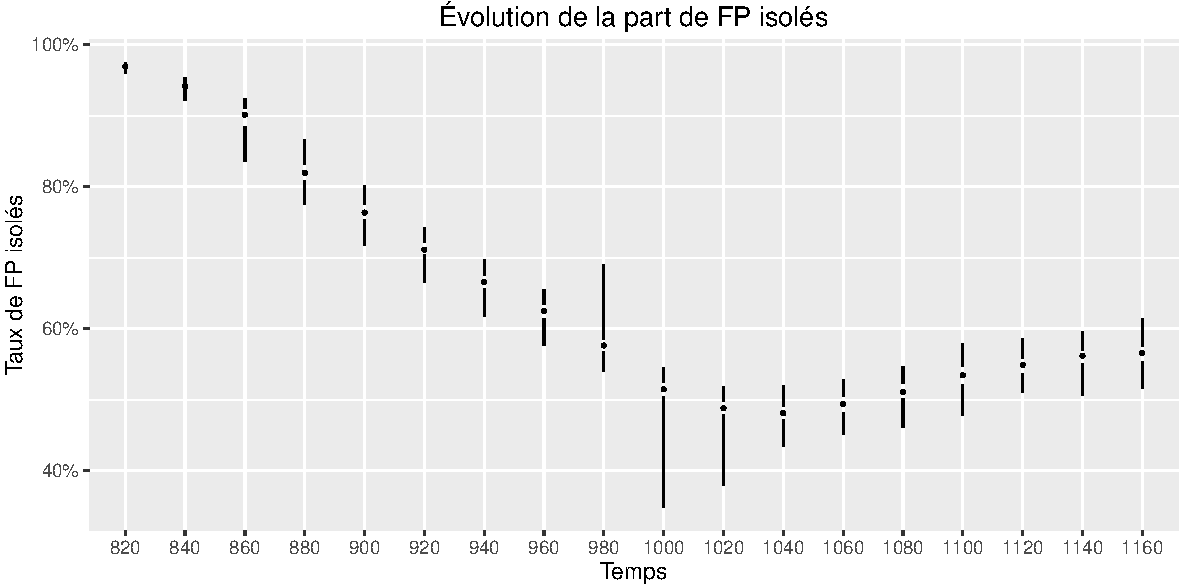
\includegraphics[width=\linewidth]{img/resultats/v0_taux_FP_isoles.pdf}
\caption{Évolution de la part des foyers paysans isolés.}
\label{fig:taux-isoles-v0}
\end{figure}

\clearpage

\subsubsection{Nombre d'agrégats}

Puisque les foyers paysans se concentrent au sein d'agrégats, il est logique d'observer l'évolution de ces derniers.
Là aussi, (\hl{objectif à définir}), on peut considérer qu'un nombre d'agrégats en fin de simulation proche de l'objectif, $200$, permet de caractériser une polarisation réussie.
Cet indicateur ne peut être lu seul, et c'est pour cela qu'il vient dans un second temps (cf. \ref{par:hierarchie_interne}, \cnameref{par:hierarchie_interne}, p.\pageref{par:hierarchie_interne}) :
en effet, un faible nombre d'agrégats peut aussi bien être révélateur d'une très faible polarisation des foyers paysans (ceux-ci restant dispersés) que d'une trop importante (un unique agrégat concentrant l'ensemble des foyers paysans par exemple).
Une fois le taux de foyers paysans dispersés connu et ces potentiels biais pris en compte, le nombre d'agrégats et son évolution nous renseigne cependant sur les dynamiques de polarisation.
D'après les connaissances expertes, on s'attend à ce que le nombre d'agrégats, très faible au départ (24 dans la version 0), suive trois phases :
une première phase de croissante lente, le temps que les mécanismes agissent sur la polarisation, suivie d'une période de croissance plus rapide, une fois que tous les foyers paysans commenceront à être suffisament attirés par les pôles pour y former des agrégats, et enfin, une nouvelle phase de croissante plus lente, une fois les foyers paysans répartis dans les agrégats existants et qui se déplaceront vers des agrégats plus importants, hiérarchisant le système de peuplement.
Cette allure d'évolution rappelle les fonctions logistiques connues par exemple pour les cycles de diffusion/adoption des innovations \hl{ref Pumain ou MN Comin}, et résulte des connaissances expertes des archéologues spécialistes de la période.

\begin{mdframed}[backgroundcolor=gray!10,footnoteinside=false]
Le nombre d'agrégats est assez satisfaisant dans la version 0 du modèle.
Il s'élève ainsi à $\textbf{187}$ en moyenne, cette dernière étant d'ailleurs stable au regard des réplications.
L'écart à l'objectif ($200$) est donc assez minime.
On a toutefois vu que le taux de foyers paysans isolé était bien trop important, et dès lors, ces agrégats sont logiquement composés de trop peu de foyers paysans.

L'observation de cet indicateur au cours du temps (\cref{fig:nombre-agregats-v0}) est quant à elle assez satisfaisante :
on retrouve bien les trois phases attendues, quand bien même le début de la croissance plus importante (vers 1000 ici) est un peu trop tardive.
Ce moment coïncide de plus avec la stagnation puis l'inversion de la courbe d'évolution de la part de foyers paysans isolés.

On peut quand même considérer que si la polarisation n'est pas assez importante, les structures qui en résultent semblent correspondre à l'empirie.
\end{mdframed}

\begin{figure}[H]
\captionsetup{width=\linewidth}
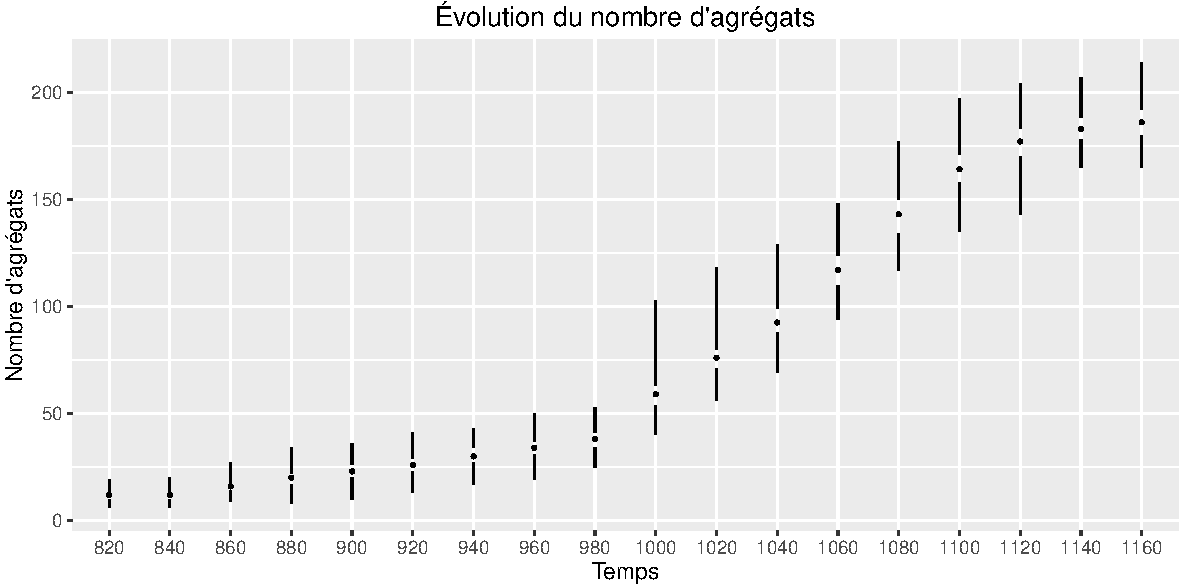
\includegraphics[width=0.5\linewidth]{img/resultats/v0_nombre_agregats.pdf}
\caption{Évolution du nombre d'agrégats.}
\label{fig:nombre-agregats-v0}
\end{figure}

\todobox{
Il y a un problème ici par rapport à ce qui a été mis dans le chapitre :
dans le chapitre TMD, on mentionne 83 agrégats en moyenne, alors que dans l'analyse de Base, il y en a 187...
}

\clearpage

\subsubsection{Nombre de pôles}\label{para:nb-poles}

Dans le modèle SimFeodal, les foyers paysans sont polarisés par des pôles d'attraction.
Pour une polarisation efficace, il est donc nécessaire que les pôles soient suffisamment nombreux, c'est-à-dire, \textit{a minima}, autant que d'agrégats attendus ($200$).
Contrairement aux agrégats, un nombre trop important de pôles ne constitue pas un problème :
en considérant que $20\%$ des foyers paysans doivent demeurer isolés en fin de simulation, il est vraisemblable qu'une partie des pôles, par exemple composés d'une église paroissiale, n'aient pas vocation à voir la constitution d'un agrégat autour d'eux.

Par ailleurs, afin de renforcer la polarisation par l'action de l'attraction différenciée -- selon le nombre de foyers paysans contenus dans chaque agrégat\footnote{\label{ftn:preferential-attachment}
L'attraction qu'exercent les pôles contenant des agrégats de population est ainsi plus forte lorsque ces derniers sont constitués d'un nombre de foyers paysans important, et moindre quand ce nombre est faible.
Cela place ce mécanisme dans une logique proche de celle de l'attachement préférentiel identifié par \cite{yule1925ii} et \cite{simon1955class}, cités par \cite[93]{schmittModelisationDynamiqueSystemes2014}) \label{ftn:attachement-preferentiel}
} --, il faut que le taux de pôles contenant un agrégat soit important, et surtout croissant au cours du temps :
comme dans l'empirie, cela est alors le marqueur que de petits pôles d'attractions, comme les églises paroissiales, parviennent à polariser suffisament de foyers paysans de leur voisinage pour aboutir à la création d'un petit agrégat, un village par exemple.

Pour un résultat satisfaisant, il faut donc que le nombre de pôles augmente régulièrement au cours de la durée de la simulation, et que le taux de pôles contenant un agrégat augmente lui aussi de manière continue.

\begin{mdframed}[backgroundcolor=gray!10,footnoteinside=false]
L'évolution du nombre de pôles est assez représentative de l'empirie dans la version 0 de SimFeodal.
On aboutit ainsi sur $\textbf{190}$ pôles en moyenne en fin de simulation, ce qui est dans le bon ordre de grandeur, quoi qu'un peu trop faible.
Ce nombre est en croissance constante à partir de 940 (\cref{fig:nombre-poles-v0}).
Ce départ quelque peu tardif peut expliquer le relatif manque de pôles en fin de simulation.

L'analyse de la constitution de ces pôles en matière d'agrégat est toutefois plus décevante :
la croissance n'est pas linéaire, stagnant entre 940 et 1000, puis à partir de 1040.
On constate ici un mauvais comportement du modèle par rapport à l'empirie :
il y a création de nombreux pôles, mais ceux-ci ne suffisent pas à polariser les foyers paysans.
On peut donc penser qu'il s'agit de nombreux pôles ruraux, par exemple composés d'une unique église paroissiale, ne suffisant dès lors pas à concentrer les foyers paysans alentours.

Dans cette dimension, comme pour l'indicateur principal qu'en est le taux de foyers paysans dispersé, l'effet de la polarisation apparaît nettement trop faible.
\end{mdframed}


\begin{figure}[H]
\captionsetup{width=\linewidth}
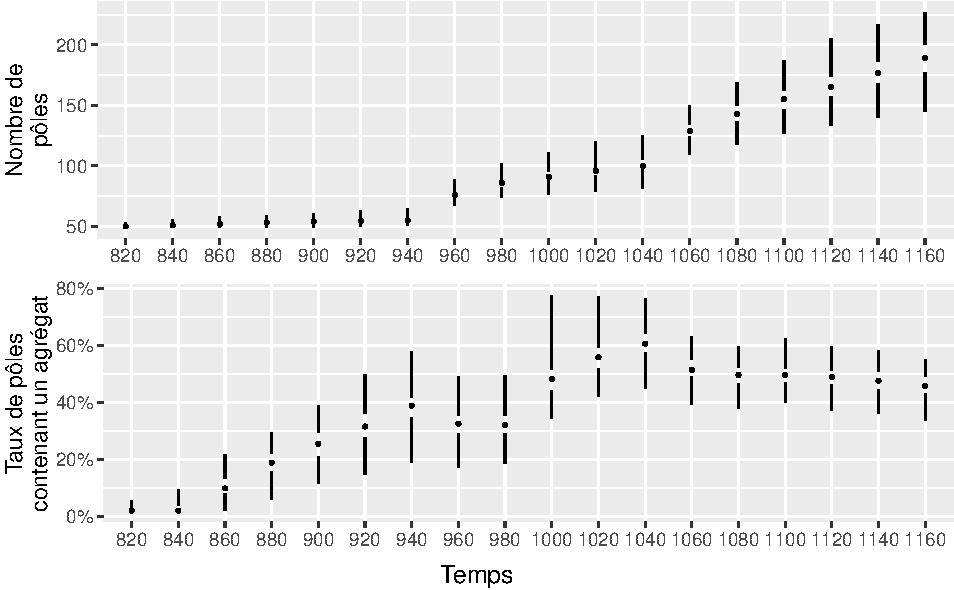
\includegraphics[width=0.5\linewidth]{img/resultats/v0_nombre_poles.pdf}
\caption{Évolution du nombre de pôles et du taux de pôles contenant un agrégat.}
\label{fig:nombre-poles-v0}
\end{figure}

\clearpage

\subsubsection{Dispersion des agrégats et pôles}\label{par:polarisation-dispersion}

Les indicateurs présentés ci-dessus avaient en commun d'être des indicateurs de sortie, générés automatiquement, et présentés sous forme d'agrégations des réplications.
Pour préciser l'analyse de la polarisation, il est toutefois nécessaire d'aborder une dimension qui n'est fondamentalement pas agrégeable dans les indicateurs de sortie :
l'espace du modèle.
Comme celui-ci est théorique et aléatoire, il n'y a aucun sens à agréger des entités différentes, par exemple des agrégats, sachant que ceux-ci occupent des localisation aléatoires et ne sont pas identifiables en tant que tels.

On ne peut cependant pas se passer d'une analyse spatiale de la répartition des pôles et agrégats afin de comprendre les dynamiques effectivement simulées par le modèle.
La distribution spatiale des agrégats et des pôles est en effet un facteur majeur de la polarisation :
s'ils sont très concentrés, les foyers paysans non présents alentours ne trouveront pas d'attracteurs à proximité, et ne seront de plus pas particulièrement affectés par l'augmentation des droits (banaux etc.) et des contraintes spatiales (proximité à une église, à un château etc.).
A l'inverse, des agrégats entièrement dispersés ne favoriseraient pas la structure spatiale hiérarchisée que l'on chercher à faire émerger.

Afin que le comportement du modèle soit satisfaisant, il faut donc que les pôles et agrégats occupent l'ensemble de l'espace du modèle, tout en présentant des zones de concentration relatives plus importantes.
Comme on ne peut agréger les représentations spatiales, il convient, pour cette analyse, de regarder individuellement un échantillon de configurations spatiales générées.

\begin{mdframed}[backgroundcolor=gray!10,footnoteinside=false]
La lecture des cartes de répartition des agrégats et des pôles de deux réplications de la version 0 (\cref{fig:cartes-agregats-v0}) va, dans l'ensemble, dans le sens de l'empirie.
On peut ainsi remarquer que ces entités ont bien tendance, au cours du temps, à se disperser dans l'espace modélisé.
En fin de simulation, tout l'espace est occupé, et on remarque même que certaines zones voient une forte concentration en agrégats, reproduisant les faits stylisés connus.
La répartition spatiale des agrégats -- et des pôles -- est donc bonne, et ne semble pas opposer d'obstacle à la polarisation attendue du système de peuplement.

Ce résultat peut cependant être nuancé par l'observation de la dynamique de cette dispersion :
on constate ainsi que la dispersion s'effectue rapidement (entre 800 et 940), et n'évolue plus vraiment après.
Ce phénomène est donc plus rapide dans cette version 0 du modèle que dans les connaissances empiriques de la région Touraine.

On peut enfin remarquer, en préalable aux dynamiques de hiérarchisation du système que l'on s'apprête à étudier, que ces sorties illustrent un manque criant de hiérarchie quant à la composition des agrégats :
on ne remarque, visuellement, que peu de différence entre les agrégats, et surtout, cette hiérarchie semble faiblir entre 1040 et 1160 (les agrégats les plus importants ont vu leur nombre de foyers paysans diminuer).
\end{mdframed}

\begin{figure}[H]
\captionsetup{width=\linewidth}
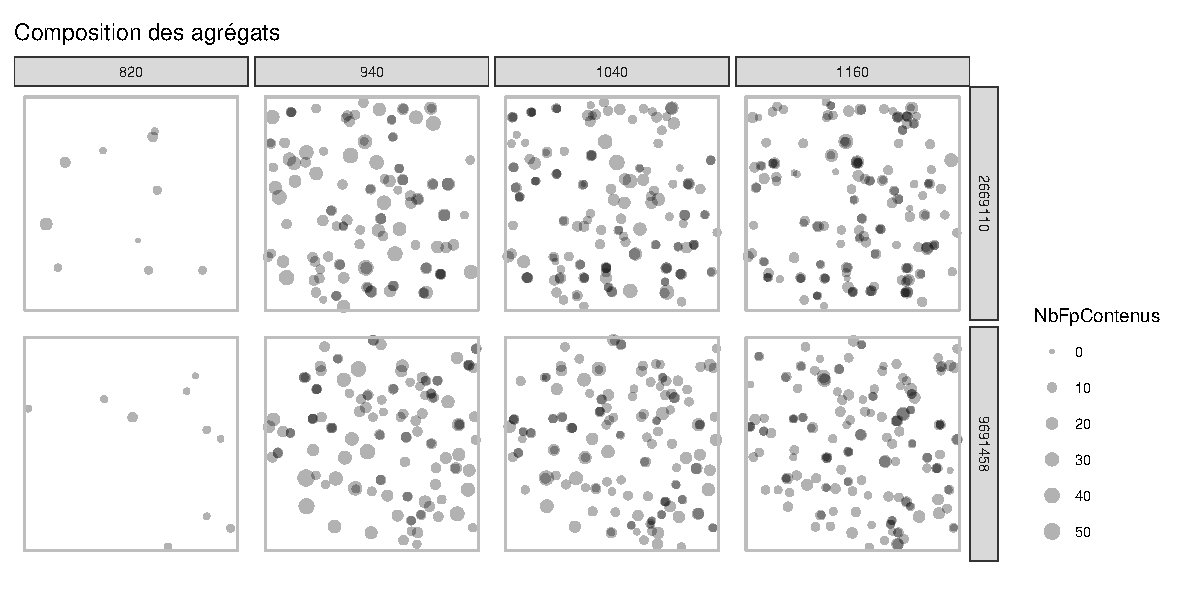
\includegraphics[width=\linewidth]{img/resultats/v0_cartes_agregats.pdf}
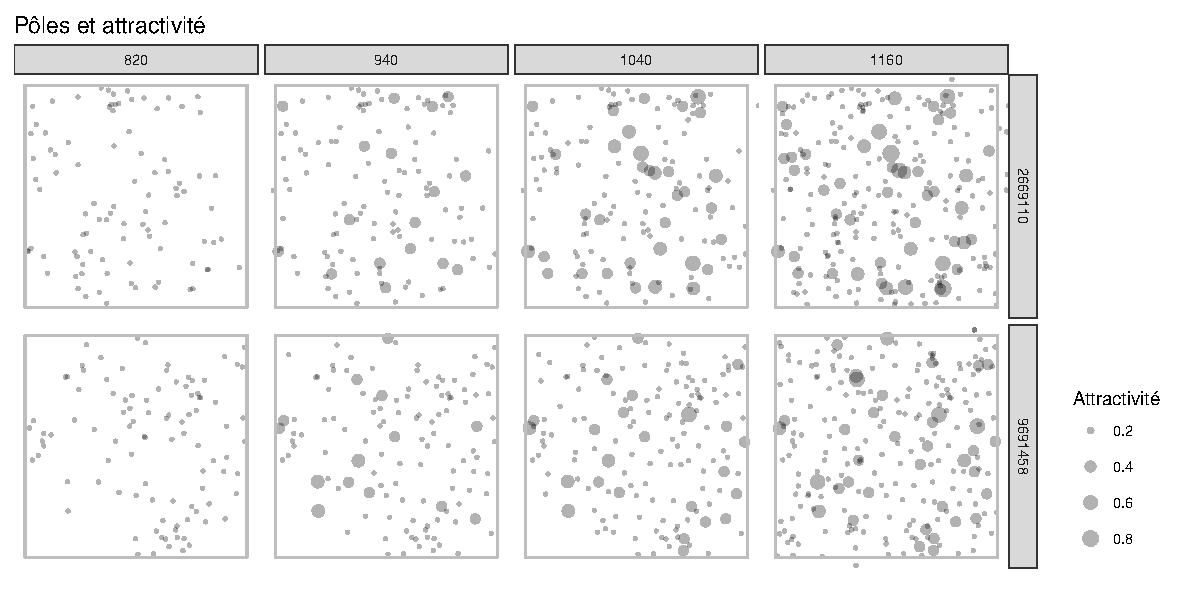
\includegraphics[width=\linewidth]{img/resultats/v0_cartes_poles.pdf}
\caption{Évolution de la répartition spatiale des agrégats et pôles, pour deux réplications.}
\label{fig:cartes-agregats-v0}
\end{figure}

\clearpage

\subsection{Évaluer la hiérarchisation du système de peuplement}

La seconde dimension de l'évaluation du modèle SimFeodal correspond à l'étude de la hiérarchisation du système de peuplement.
On déduit en effet des connaissances empiriques une forte hiérarchisation du système de peuplement sur la période, et plus généralement, des entités présentes.
On passe ainsi, en 800, d'un habitat dispersé dans lequel coexistent quelques agrégats de taille uniforme, à un habitat concentré dans des agrégats de taille très hétérogènes à la fin du XIIème siècle.
La distribution des tailles des agrégats est estimée par les connaissances expertes, toutes proportions gardées, comme assez proche des distributions observées aujourd'hui dans les systèmes de peuplement.
On souhaite ainsi que les agrégats modélisés suivent une distribution approchant la distribution log-normale.

Par extension, et là encore d'après les connaissances thématiques, l'ensemble des entités doit aussi suivre le même type de forme.
Par exemple, les pôles, tant en terme d'attractivité que de composition, doivent aussi montrer une hiérarchie du même ordre, ainsi que les seigneurs -- à travers leur puissance, au moins pour les petits seigneurs --, ou encore les paroisses, par le nombre de paroissiens qu'elles desservent.

Comme pour l'étude de la polarisation, on peut définir un indicateur principal de cette hiérarchisation du système de peuplement :
la forme de la distribution de la composition en foyers paysans des agrégats.

De la même manière que pour la polarisation, les indicateurs secondaires ont aussi pour but de préciser cet indicateur principal, et en particulier d'analyser les moteurs de cette hiérarchisation du peuplement.
On a en effet choisi d'observer plutôt la hiérarchisation des autres types d'entités -- pôles, seigneurs, paroisses --, pour vérifier qu'elles accompagnent et/ou entraînent bien la hiérarchisation des agrégats.
La hiérarchie des pôles, par exemple, a une influence directe sur l'attraction effectuée sur les foyers paysans (polarisation) et sur la hiérarchisation des agrégats :
par effet d'attraction différenciée (voir la note de bas de page \ref{ftn:attachement-preferentiel} \cpageref{ftn:attachement-preferentiel}), des agrégats plus importants se constituemouvementnt autour des pôles les plus importants.

Comme pour la polarisation, l'analyse de la capacité du modèle a reproduire la hiérarchisation du système de peuplement se fait donc en deux temps :
en premier lieu, on évalue cette capacité à l'aide de l'indicateur principal, puis on précise cette qualification et on essaie de l'expliquer à l'aide des indicateurs secondaires.


\subsubsection{Hiérarchie des agrégats}

L'indicateur principal est un indicateur agrégé, correspondant à la forme de la distribution des agrégats mesurés par le nombre de foyers paysans qui les composent.
Cet indicateur est classique dans l'analyse des systèmes de peuplement, et il est courant de l'observer par le biais d'un indicateur agrégé simple, correspondant à la loi rang-taille.
On observe pour cela le modèle statistique, ou sa représentation graphique tout du moins, mettant en relation le logarithme de la taille des individus (le nombre de foyers paysans composant chaque agrégat ici) et le logarithme du rang de cet individu.
Comme pour toute régression linéaire, on peut alors quantifier l'ajustement du modèle grâce au coefficient de détermination ($R^2$), et spécifier la pente de la courbe, représentant le degré de hiérarchie, à travers le coefficient directeur ($a$ dans la formule $y = ax + b$).

Dans le cas de SimFeodal, le faible nombre d'agrégats ainsi que la variabilité de leurs tailles rend difficile cette analyse quantifiée, le coefficient directeur, par exemple, étant très sensible aux faibles effectifs.
On utilise toutefois la représentation graphique décrite comme un indicateur majeur de la hiérarchie des agrégats.

Du point de vue des connaissances empiriques, la courbe doit ainsi voir sa pente augmenter avec le temps, tout en devenant plus convexe, ce qui représente la \og longue traine\fg{} des petits agrégats, empiriquement observée dans toutes les distributions de systèmes de peuplement.

Avec une autre représentation graphique du même phénomène, en discrétisant les agrégats selon leur taille et en dénombrant le nombre d'agrégats de chaque classe, on peut aussi avoir une vision plus synthétique (car moins exhaustive) de la forme de la distribution.
On doit alors obtenir un nombre décroissant d'agrégats à mesure que la classe représente un nombre élevé de foyers paysans.

\todobox{
Ça vaudrait peut-être le coup, pour chaque indicateur présenté sous forme graphique (évolution ou forme), de faire un graphique théorique (une sorte de courbe parfaite) de ce que l'on souhaite observer.
}

\begin{mdframed}[backgroundcolor=gray!10,footnoteinside=false]
La version 0 de SimFeodal présente une hiérarchisation des agrégats nettement trop faible.
La courbe rang-taille (\cref{fig:rt-agregats-v0}) est ainsi trop faiblement pentue, et présente une forme trop linéaire :
la convexité due à la longue traine n'est pas assez visible, en raison sans doute de trop faibles valeurs  en haut de la hiérarchie, qui ne \og tire\fg{} alors pas assez la distribution.
Ce résultat de simulation est d'autant plus perturbant que son évolution est éloignée de l'empirie :
on remarque en effet que la distribution se hiérarchise bien entre 800 et 1020, présentant à cette date une allure très satisfaisante.
Pourtant, après cette période, les agrégats voient leur hiérarchie diminuer nettement et les agrégats les plus peuplés diminuer en taille.

On constate le même décrochage dans la discrétisation des agrégats (\cref{fig:compo-agregats-v0}), où on remarque de plus que la hiérarchie la plus proche de l'attendu, où la position des classes suivrait une ligne droite, semble se dessiner entre 940 et 1040.
En 1040, et plus encore en 1160, la proportion d'agrégats de taille moyenne et haute (de 30 à 100, et de plus de 100 foyers paysans) est trop faible, et pas assez hiérarchisée.

\end{mdframed}

\begin{figure}[H]
\captionsetup{width=\linewidth}
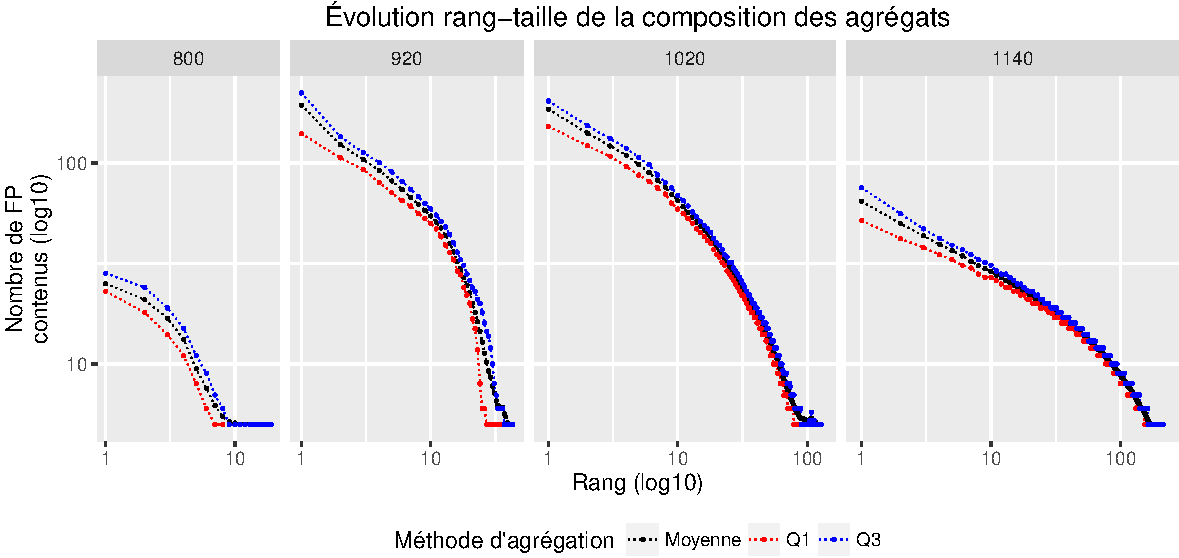
\includegraphics[width=.8\linewidth]{img/resultats/v0_rt_agregats.pdf}
\caption{Évolution de la courbe rang-taille des agrégats.}
\label{fig:rt-agregats-v0}
\end{figure}

\begin{figure}[H]
\captionsetup{width=\linewidth}
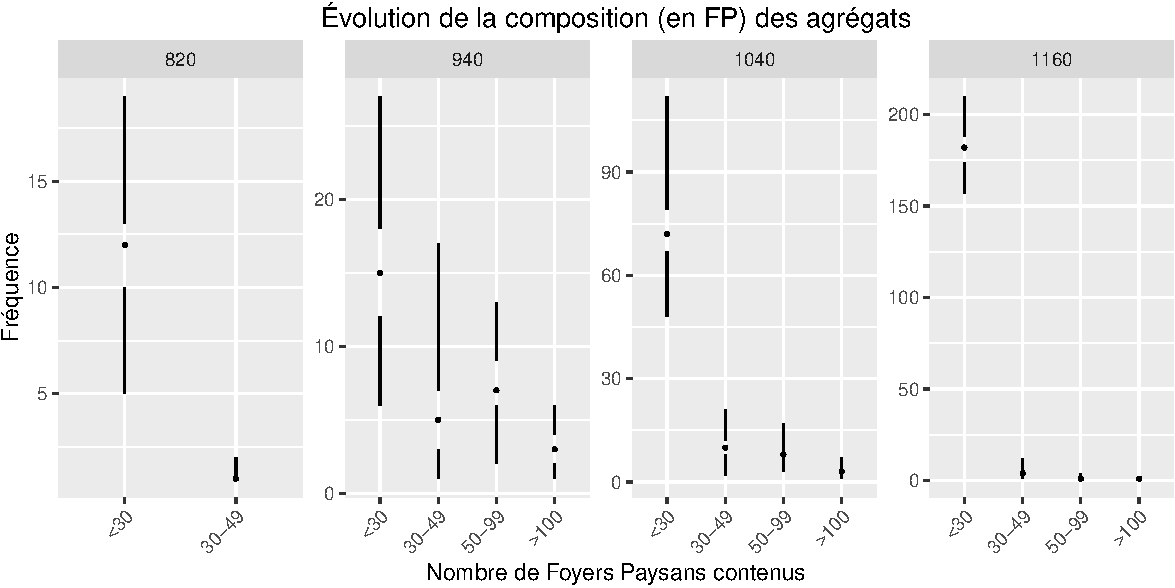
\includegraphics[width=.8\linewidth]{img/resultats/v0_compo_agregats.pdf}
\caption{Évolution de la composition des agrégats.}
\label{fig:compo-agregats-v0}
\end{figure}

\clearpage

\subsubsection{Hiérarchie des pôles}

La hiérarchie des agrégats donne une bonne vision agrégée de la hiérarchisation du système de peuplement dans son ensemble.
Pour autant, afin d'appréhender la dynamique de cette dimension, il est là encore nécessaire d'observer le comportement des composantes qui provoquent cette hiérarchisation.
En effet, une forte hiérarchie des pôles entraînera une attractivité des foyers paysans très inégale \footnote{En raison des logiques d'attachement préférentiel, voir la note de bas de page \ref{ftn:preferential-attachment} page \pageref{ftn:preferential-attachment}.} De plus, comme indiqué plus haut, on cherche à obtenir une forte hiérarchi)e pour les différents types d'agents du modèle.
L'observation de la hiérarchie des pôles est donc importante pour évaluer le modèle SimFeodal.
Pour déterminer cette hiérarchie, on peut se fier à deux indicateurs complémentaires :
le nombre d'attracteurs composant chaque pôle et l'attractivité de ces derniers.
Ces indicateurs de sortie sont proches, mais apportent pourtant une vision légèrement différente :
étant donné que chaque attracteur influe différemment, selon son type, sur l'attractivité globale d'un pôle, l'information sur l'attractivité et sur la composition ne sont pas redondantes, bien que fortement corrélées.
On aurait pu présenter une information plus détaillée quant à cette composition, par exemple en différenciant le nombre de chacun des types d'attracteurs de chaque pôle, mais le nombre de combinaisons possible aurait rendu cette information confuse.

À partir des connaissances expertes qui guident l'évaluation de SimFeodal, on cherche à obtenir, pour ces deux indicateurs, une courbe d'allure similaire, c'est-à-dire une courbe décroissante, avec bien plus de pôles mineurs (faible attractivité ou nombre d'attracteurs) que de pôles plus importants.
On cherche de plus à ce que cette courbe présente une allure log-normale, et donc que la proportion de pôles décroisse fortement à mesure que leur importance augmente.


\begin{mdframed}[backgroundcolor=gray!10,footnoteinside=false]
Dans l'ensemble, on peut remarquer sur les deux indicateurs de la \cref{fig:compo-poles-v0} que les pôles, dans cette version 0, sont très hiérarchisés.
La tendance \og évolutive va dans le bon sens :
depuis une quasi-uniformité en 820, des pôles plus importants apparaissent et semblent se renforcer au cours du temps.
On retrouve aussi, en observant les axes des ordonnées, la croissance du nombre de pôles identifiée plus haut (\ref{para:nb-poles}, \cnameref{para:nb-poles}, p. \pageref{para:nb-poles}) :
de nouveaux pôles apparaissent tout au long de la simulation, et restent majoritairement peu importants, quand les pôles ayant commencé à se renforcer tôt continuent dans cette tendance.

En fin de période, les pôles sont très hiérarchisés, aussi bien en matière de composition que d'attractivité.
Ils le sont même plus que ce que les connaissances expertes laissent entendre :
au delà de $0.66$ en attractivité ou de $4$ attracteurs, on ne dénombre plus qu'un unique pôle de chaque importance, là où on attendrait que cette courbe continue plutôt à décroitre.
De plus, ces courbes montrent la variation des réplications de la version 0.
Dès lors, on peut considérer que ces pôles majeurs ne sont en fait qu'un unique pôle (le plus souvent) d'importance variable selon les réplications, mais dans tous les cas d'importance bien supérieure aux pôles qui arrivent juste après dans le classement.
Cette macrocéphalie ne correspond pas aux observations empiriques, d'autant que rappelons-le, la ville de Tours n'est pas modélisée dans SimFeodal.


\end{mdframed}

\begin{figure}[H]
\captionsetup{width=\linewidth}
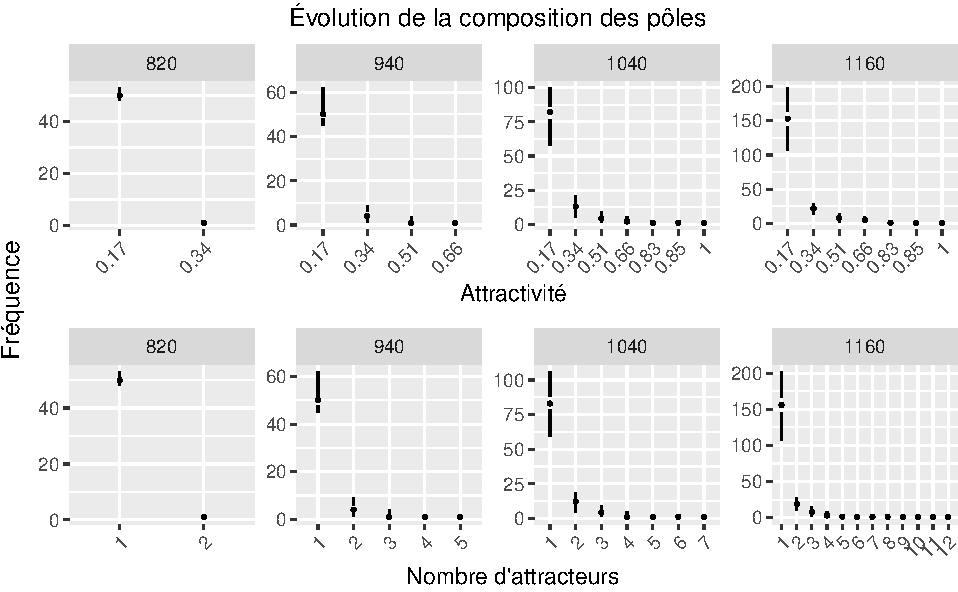
\includegraphics[width=\linewidth]{img/resultats/v0_compo_poles.pdf}
\caption{Évolution de la composition et de l'attractivité des pôles\protect\footnotemark{}.}
\label{fig:compo-poles-v0}
\end{figure}
\footnotetext{\hl{Les figures ne sont pas en log-log (ou log-lin) et on ne voit donc pas vraiment le haut de la hiérarchie.
Peut-être faudrait-il changer ces axes, mais ça complexifiera la lecture pour les archéos/lecteurs non habitués aux axes log}}

\clearpage

\subsubsection{Hiérarchie des paroisses}\label{par:hierarchie-paroisses}

A l'instar des pôles, on attend aussi des ressorts paroissiaux d'être hiérarchisés.
La période modélisée voit ainsi apparaître ces paroisses qui auront un rôle majeur dans la fixation du peuplement, et, pré-figurant le maillage communal, ont un double rôle de desserte efficace\footnote{C'est-à-dire desservir de manière optimale la plupart de la population.} et équitable\footnote{C'est-à-dire faire en sorte que même les populations les plus isolées aient un accès aussi rapide que possible à une église paroissiale.}.
En effet, avec la volonté d'encadrement et de prélèvement de l'Église sur la population, de nouvelles paroisses apparaissent pour desservir au mieux leurs potentielles ouailles.
Une structure double en résulte :
dans les zones les moins denses, le maillage est régulier mais lâche, de manière à minimiser le nombre d'églises paroissiales tout en s'assurant que chacun puisse y accéder dans un temps raisonnable\footnote{Cette distance-temps évolue au cours du temps, en fonction de l'accroissement de la fréquence de l'obligation de fréquentation des églises paroissiales.}.
Il y a donc un certain nombre d'églises paroissiales desservant peu de paroissiens.
Au contraire, dans les zones les plus denses, et en particulier au sein des petites villes naissantes, l'objectif est d'être au plus près des résidents tout en garantissant à chacun de pouvoir assister aux différents offices :
il y donc une croissance du nombre d'églises paroissiales proches les unes des autres, visant à accompagner un encadrement maximum de la population, ainsi, avec une logique concurrentielle de ce clergé féodal, qu'à capter l'importante source de revenus qu'assure la collecte de la dîme.
Cette logique concurrentielle doit aussi permettre de restreindre le nombre de foyers paysans desservis par une unique paroisse.

On s'attend donc à avoir une courbe hiérarchisée dans la lignée d'une courbe log-normale, mais avec toutefois un double seuil minimal (l'effet de \og longue traîne\fg{}), autour des paroisses \og rurales\fg{} peu peuplées (moins de 10 foyers paysans désservis) et des paroisses du bas de la hiérarchie classique, peuplées de 10 à 40 foyers paysans\footnote{D'après les valeurs des paramètres \texttt{nb\_min\_paroissiens} et \texttt{nb\_max\_paroissiens}}).

\todobox{ici, impérativement, il faudra mettre un graphique schématique de ce qu'on attend.}

\begin{mdframed}[backgroundcolor=gray!10,footnoteinside=false]
En fin de simulation de cette version 0, la hiérarchie des paroisses est plutôt satisfaisante.
On y retrouve en effet une forte hiérarchie, peut-être même légèrement trop importante.
Il ne devrait ainsi par y avoir de paroisse composée de plus de $100$ foyers paysans en fin de simulation, et la courbe présente une pente trop importante (celles de 940 ou 1040 sont ainsi plus conformes aux attentes).
Pour autant, on remarque bien un effet de hiérarchisation au cours du temps, ainsi qu'un accroissement du nombre de petites paroisses, montrant que la dynamique, bien que non ajustée, s'inscrit bien dans la dynamique observée empiriquement.
(\cref{fig:compo-paroisses-v0})
\end{mdframed}

\begin{figure}[H]
\captionsetup{width=\linewidth}
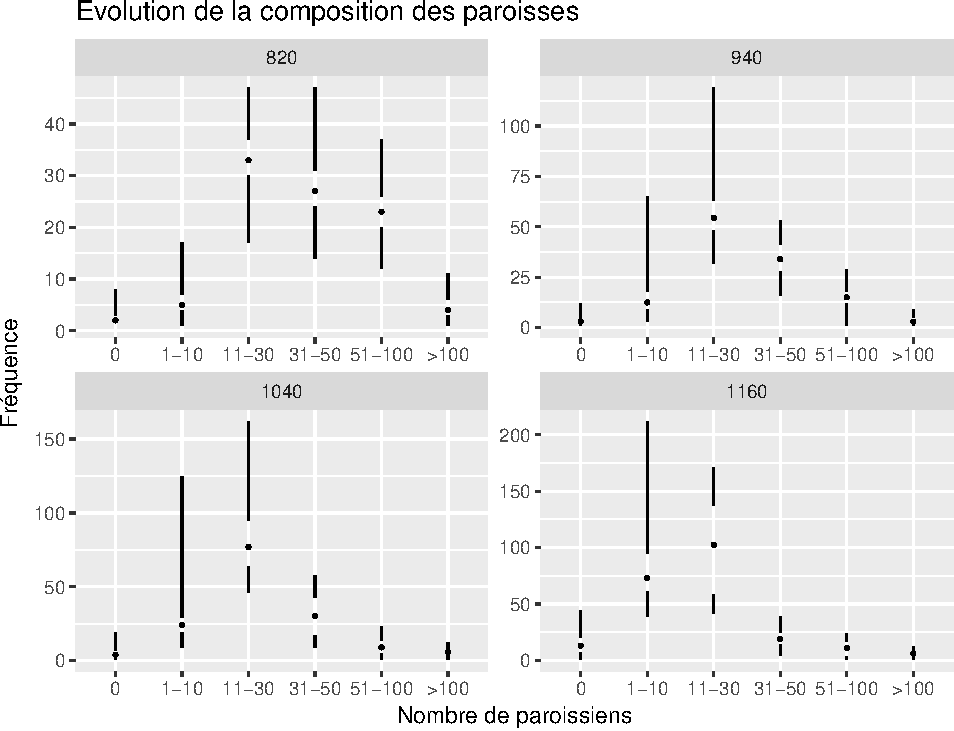
\includegraphics[width=\linewidth]{img/resultats/v0_compo_paroisses.pdf}
\caption{Évolution de la composition des paroisses.}
\label{fig:compo-paroisses-v0}
\end{figure}

\clearpage

\subsection{Évaluer la fixation et la dissémination du peuplement}


La dernière dimension étudiée par SimFeodal est moins définie que les précédentes.
On y observe ainsi la fixation du système de peuplement au sein du maillage naissant que constituent les paroisses.
Cette notion de fixation pose problème par rapport à l'ensemble des indicateurs de sortie déployés jusqu'ici.
En effet, SimFeodal est un modèle fondé sur un temps discret :
on y observe, à chaque itération, le résultat des processus modélisés.
On peut y observer une fixation d'un pas de temps par rapport à l'autre, par exemple en constatant qu'un agrégat constitué en 820 semble être toujours présent en 840.
On peut de plus considérer que cet agrégat présente les mêmes caractéristiques au deux dates, en matière de localisation et de population.
L'agrégat est donc stable dans le temps.
L'échelle d'analyse mobilisée dans les indicateurs précédents -- au niveau agrégé des agrégats, voir du système d'agrégats -- pourrait donc s'appliquer ici aussi.
Pourtant, quand on parle de fixation des foyers paysans, ce qui est observé empiriquement, il n'est pas question d'agrégats, mais des entités les composant, c'est-à-dire les foyers paysans.
Ceux-ci ne sont pas observés directement quand on remarque que les agrégats semblent stable :
on approche là à la différence entre un état stable et un état stationnaire.
La relative stationnarité des agrégats dans le temps n'est ainsi pas garante de stabilité de leurs composantes :
deux foyers paysans oscillant d'un agrégat à un autre, dans un mouvement opposé, produiraient ainsi une stationnarité de ces agrégats, mais, en se déplaçant, ils ne satisferaient pas au critère de fixation.
Il y a donc un problème de changement d'échelle pour observer la fixation des foyers paysans :
il n'est plus possible de raisonner à l'échelle des agrégats, et il faut se concentrer sur celle des foyers paysans.

Cette échelle pose un autre problème :
les foyers paysans sont très nombreux ($4000$ dans la version 0) et se déplacent.
Ils se déplacent de plus selon des modalités très différentes (\hl{Faire ref aux mécanismes de déplacement du chapitre 2}), rendant complexe la caractérisation des mouvements de chacun et plus encore celle d'une agrégation de ces catégories.

Pour ces raisons, la production d'indicateurs synthétiques spatiaux -- une ou plusieurs cartes -- ne suffirait pas à communiquer une information intelligible sur l'éventuelle fixation des foyers paysans.
Il nous faut donc faire appel à des \og proxys\fg{}, non spatiaux, pour évaluer la fixation des foyers paysans.

A cet effet, on a retenu des indicateurs relatifs aux déplacements des foyers paysans et à leur raison :
combien de foyers paysans se déplacent à chaque pas de temps (moins il y a de déplacement, plus la fixation est importante) ? Quelles sont les modalités de ces déplacements (un déplacement entre deux agrégats lointains n'a pas les mêmes conséquences en terme de stabilité qu'un déplacement minime au sein d'un même agrégat) ? Ou encore, comment évolue la satisfaction des foyers paysans, et avec celle-ci, la probabilité de se déplacer ?

Ces indicateurs permettent d'évaluer la capacité du modèle à reproduire la fixation des foyers paysans.
Pour autant, la contrainte est ici double :
on recherche une fixation, mais celle-ci est, empiriquement, supposée se dérouler et se voir renforcer par la mise en place du maillage paroissiale qui doit servir de support à la nouvelle configuration spatiale émergente.

On s'appuiera donc aussi sur des indicateurs relatifs à cet espace support constitué par les paroisses :
leur nombre, leur dispersion dans l'espace et l'efficacité de la desserte qu'elles assurent.

\paragraph*{}Notons que contrairement aux deux précédents dimensions d'analyse, nous n'établissons ici pas de hiérarchie nette entre les indicateurs.
Cette étude de la fixation est moins facilement appréhendable que celle de la polarisation ou de la hiérarchisation et les indicateurs qui la caractérisent apportent une complémentarité de points de vue plus qu'un affinement de l'évaluation de cette dynamique.
Dès lors, les indicateurs présentés ci-après ne peuvent être catégorisés en indicateurs principaux et secondaires.
On retrouvera cependant cette hiérarchie d'évaluation au sein des indicateurs, par exemple en suivant l'ordre des graphiques présentés.
Par exemple, pour évaluer la fixation des foyers paysans, on observera d'abord le résultat produit (nombre de déplacements) avant d'entrer dans le détail de sa composition (types des déplacements).


\subsubsection{Déplacement des foyers paysans}

Le déplacement des foyers paysans est l'élément moteur de SimFeodal :
c'est par le déplacement individuel de chacun des foyers paysans que la configuration spatiale évolue.
Les déplacements affectent donc chacune des dimensions d'analyse -- polarisation, hiérarchisation et fixation --, mais c'est au sein de cette dernière qu'il est le plus intéressant de les observer.
Il est en effet attendu que de nombreux déplacement surviennent, afin que le système de peuplement puisse se structurer, mais pour autant, il est aussi nécessaire que ces déplacements tendent à diminuer au cours du temps, une fois le système en voie de stabilisation.

On pourrait donc attendre que les déplacements suivent une courbe négative (linéaire ou non) tendant vers 0, impliquant une absence de déplacements en fin de période.
Pour autant, le mécanisme de déplacement est sans doute l'un des plus complexes du modèle, et on ne peut l'appréhender aussi simplement.

En premier lieu, les mécanismes de SimFeodal différencient deux types de déplacements (\hl{Faire ref à chap2}) :
les déplacements locaux (dans un rayon de $2500$m dans la version 0) et les déplacements lointains.

\begin{itemize}
\item Les déplacements locaux visent à faire s'agréger des foyers paysans dispersés autour de pôles présents à proximités.
Ce mécanisme peut être présent sur toute la durée de la simulation, sur un effectif faible.
En effet, cet effet d'agrégation locale permet \og d'optimiser\fg{} la répartition spatiale des agrégats, en renforçant leur hiérarchie et en faisant fusionner des agrégats qui seraient très proches les uns des autres.
Pour autant, dans un objectif de fixation du peuplement, il est nécessaire de veiller à ce que les foyers paysans ne soient pas amenés à se déplacer localement de manière continuelle, par exemple en faisant des allers-retours entre des pôles ou agrégats spatialement proches.

\item Les déplacements lointains servent un autre rôle :
un foyer paysan qui ne serait pas en mesure d'augmenter sa satisfaction localement -- faute de pôles suffisamment attractifs dans le voisinage -- a une probabilité de se déplacer vers un agrégat situé n'importe où dans l'espace modélisé.
Le modèle est très sensible à ce mécanisme qui agit comme une perturbation forte dans la structure spatiale du peuplement.
Ce mécanisme \og de dernier recours\fg{} ne doit être employé que rarement, en cas de situations où des foyers paysans seraient trop isolés pour pouvoir s'agréger localement.
C'est notamment le cas pour les foyers paysans nouveaux arrivants, via le mécanisme de renouvellement (\hl{ref dans chap 2}), qui peuvent se voir localisés n'importe où dans l'espace du modèle.
\end{itemize}

Pour ajouter à la complexité du mécanisme, et donc de l'évaluation de cet indicateur qu'est le nombre de déplacements au cours du temps, rappelons que différentes contraintes temporelles viennent bouleverser, à dessein, le comportement des foyers paysans.
En particulier, entre 950 et 1050, les modalités d'évaluation de la satisfaction deviennent plus strictes (\hl{Voir dans chap2, frise}).
Cela engendre nécessairement une plus forte propension des foyers à se déplacer.

Si les connaissances empiriques d'un tel niveau de finesse ne sont pas disponibles, on peut tout de même avoir des attentes quant au comportement attendu du modèle.
Au regard des éléments décrits plus haut, on peut ainsi chercher à ce que l'évolution des déplacements suive plusieurs rythmes au cours du temps :
\begin{enumerate}
\item Dans une première phase, du début de la simulation jusqu'aux perturbations débutant en 950 :
quelques déplacements lointains marginaux ($\approx 5$\% à $10$\%), stables au cours du temps ; et de plus nombreux (au moins $\approx 30$\%) déplacements locaux menant à la constitution de petits agrégats locaux.
Les déplacements locaux doivent diminuer au cours du temps, une fois les agrégats constitués.
\item Pendant la deuxième phase, entre 950 et 1050, les nombreuses perturbations devraient voir une nette augmentation des déplacements locaux, et dans une moindre mesure lointains, prémices à la constitution d'agrégats plus hiérarchisés.
\item Après ces perturbations, on devrait retrouver le niveau de déplacement de la seconde période, et là aussi, tendre vers une diminution des déplacements locaux, le système se stabilisant à l'approche de la fin de la période.
\end{enumerate}

Tout au long de cette période, on cherche de plus à ce que les foyers paysans soient polarisés, c'est-à-dire ici, qu'ils se regroupent dans des agrégats de population.
Parmi les modalités de déplacement, un autre indicateur utile est ainsi l'observation des provenances et destinations des foyers paysans qui se déplacent :
plus les foyers paysans originellement dispersés auront tendance à rejoindre des agrégats, plus la simulation sera satisfaisante au regard des hypothèses empiriquement émises.


\begin{mdframed}[backgroundcolor=gray!10,footnoteinside=false]
Dans cette version 0 de SimFeodal, il apparaît en premier lieu que les déplacements sont trop peu nombreux (\cref{fig:nb-deplacements-v0}).
Les déplacements lointains sont à peu près dans les proportions attendues, mais les déplacements locaux sont trop peu nombreux.
Surtout, les trois phases attendues ne se retrouvent pas sur ces sorties.
On y remarque bien l'impact des perturbations, mais celles-ci ne font qu'augmenter la part de déplacements, laquelle reste stable avant et après ces perturbations.
La version 0 de SimFeodal n'est donc pas satisfaisante en termes de stabilisation et de fixation des foyers paysans.
L'observation des modalités de déplacement (\cref{fig:type-deplacements-v0}) montre certes une part croissante de déplacements \og Isolé -> Agrégé\fg{}, mais dans des proportions là aussi trop faibles passé le tout début de la simulation.
\end{mdframed}

\begin{figure}[H]
\captionsetup{width=\linewidth}
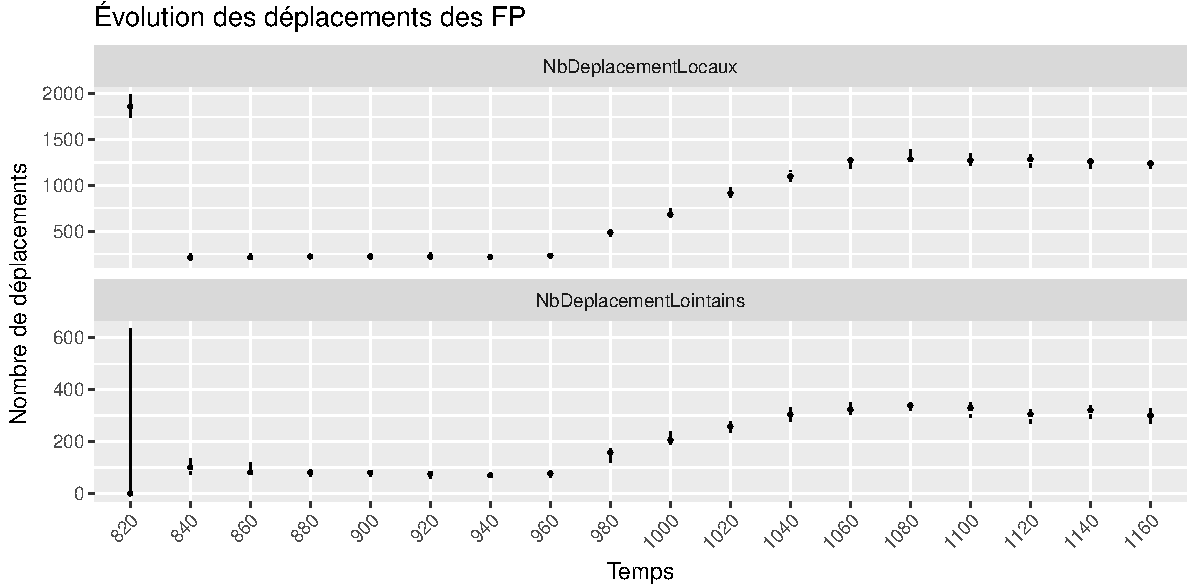
\includegraphics[width=\linewidth]{img/resultats/v0_nombre_deplacements.pdf}
\caption{Évolution du nombre de déplacement des foyers paysans.\\
\todobox{Mettre le graphique en relatif}}
\label{fig:nb-deplacements-v0}
\end{figure}



\begin{figure}[H]
\captionsetup{width=\linewidth}
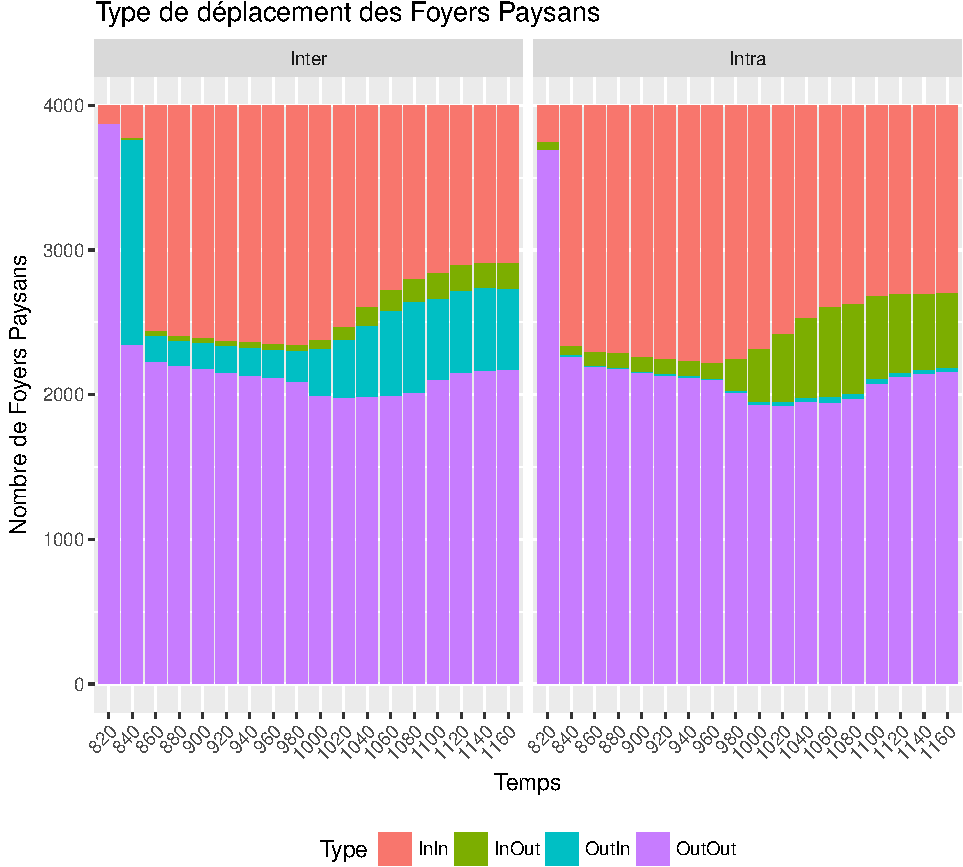
\includegraphics[width=\linewidth]{img/resultats/v0_types_deplacements.pdf}
\caption{Évolution des types de déplacement des foyers paysans.\\
Inter : Déplacement depuis le pas de temps précédent vs Intra :
déplacement au sein d'un même pas de temps.
\todobox{Ne garder que l'inter et mettre le graphique en relatif}\\
%	- InIn : Le FP était dans un agrégat au pas de temps précédent, et est dans un agrégat à ce tour (quel qu'il  soit, ça peut être le même ou un autre).\\
%	- InOut : Le FP était dans un agrégat au pas de temps précédent, et est isolé à ce tour\\
%	- OutIn : Le FP était isolé, et est maintenant dans un agrégat\\
%	- OutOut : Le FP était isolé, et l'est toujours\\
%On constate donc que les déplacements au sein d'un tour tendent à isoler les FP, grosso modo dans le même temps et les mêmes proportions que la stabilisation du taux de FP isolés.
}
\label{fig:type-deplacements-v0}
\end{figure}

\clearpage

\subsubsection{Satisfaction des foyers paysans}

On a vu dans les deux indicateurs précédents que les déplacements des foyers paysans sont très affectés par leur niveau de satisfaction.
Pour comprendre ces déplacements, il est donc utile d'observer en détail l'évolution de la satisfaction qui les provoquent.

La satisfaction ne saurait être résumée en un simple indicateur de fixation, tant son rôle est prépondérant dans une large partie des mécanismes du modèle.
Pourtant, mobilisé ici, cet indicateur apporte un éclairage différent.
Il permet ainsi de préciser les indicateurs précédents en donnant une explication à leur éventuelle mauvaise réponse aux attentes.

Ainsi, une satisfaction globalement trop élevée ne serait pas assez motrice à des déplacements, résultant en une polarisation faible.
Au contraire, une satisfaction globalement faible engendrerait une très forte mobilité, par exemple sous forme de mouvements pendulaires, d'où une absence de fixation du peuplement.
Comme pour les déplacements, on attend, depuis les connaissances empiriques, qu'il y ait trois phases dans l'évolution de cette satisfaction :
(1) une première phase, jusqu'en 950, où les foyers paysans sont globalement satisfaits, et le sont de plus en plus à mesure qu'ils s'agrègent ;
(2) une seconde phase, entre 950 et 1050, où les restrictions fortes (distance à un château, à une église paroissiale) auront pour effet de violemment abaisser le niveau de satisfaction ;
et enfin, (3) une dernière phase où, passées les perturbations, le niveau de satisfaction tend à remonter doucement, sous l'effet de l'agrégation et de la constitution généralisées de communautés paysannes et de la construction de châteaux et de nouvelles églises paroissiales.

\begin{mdframed}[backgroundcolor=gray!10,footnoteinside=false]
Au vu des résultats de la version 0 de SimFeodal illsutrés dans la \cref{fig:satisfaction-fp-v0}, on constate que les trois phases attendues sont bien présentes.
La perturbation en milieu de période est très forte, mais pourtant, le niveau de satisfaction général reste très élevé (à toute date, plus de $80$\% des foyers paysans ont une satisfaction supérieure à $0.5$).
Avec ce niveau de satisfaction et les mécanismes de déplacement de cette version 0, seuls les foyers paysans à proximité de très gros pôles (au moins un gros château et plusieurs églises paroissiales) pourront se déplacer localement.
Et pour peu qu'il y ait plusieurs pôles importants à proximité, ils oscilleront entre les deux, gonflant artificiellement le nombre de déplacements locaux.
L'observation de cet indicateur confirme que le niveau de déplacement est trop faible et ne présente pas l'allure attendue, tout en donnant une explication à la mauvaise fixation du peuplement observée.
\end{mdframed}

\begin{figure}[H]
\captionsetup{width=\linewidth}
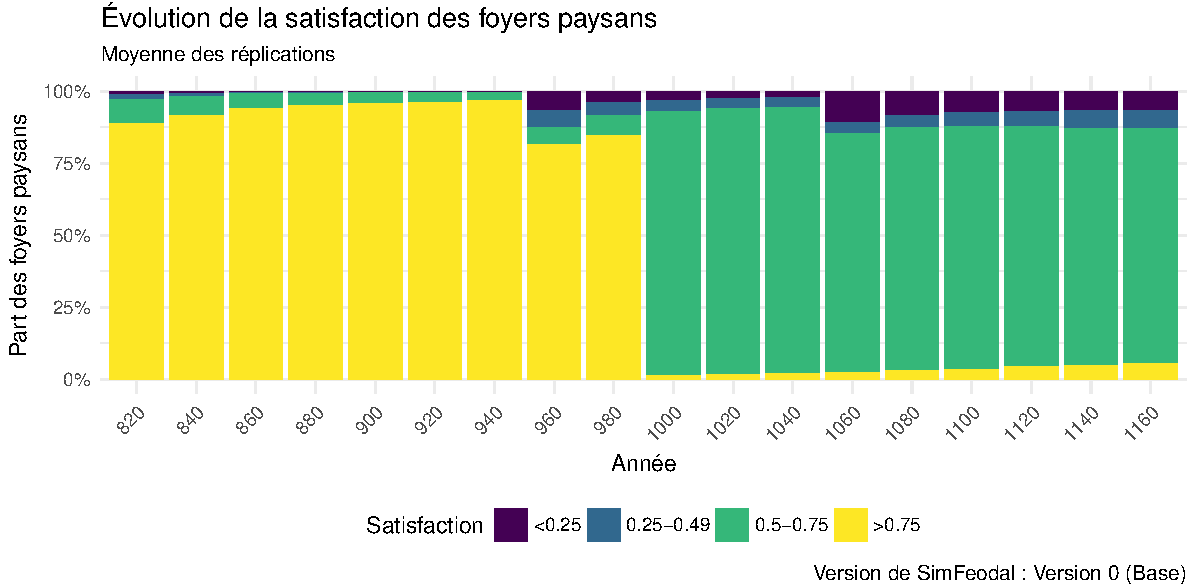
\includegraphics[width=0.95\linewidth]{img/resultats/v0_satisfaction_fp.pdf}
\caption{Satisfaction des foyers paysans}
\label{fig:satisfaction-fp-v0}
\end{figure}

\clearpage

\subsubsection{Nombre et dispersion des paroisses}

Tout au long de la période, de nouvelles églises paroissiales sont créées (\hl{cf. mécanisme dans chap. 2}) et viennent renforcer l'encadrement des foyers paysans.
L'évolution du maillage constitué par les ressorts paroissiaux représente donc l'évolution de la structure spatiale des foyers paysans.
Pour que les foyers paysans soient satisfaits, il faut, à partir de 950, qu'ils soient suffisament proches d'une église paroissiale
Celles-ci constituent donc, à mesure de l'avancement de la période, des pôles qui vont aider à la fixation des foyers paysans.
Il est donc légitime d'observer la croissance du nombre et la répartition des paroisses telles que simulées dans le modèle SimFeodal.

Sur un plan purement numéraire, plus les paroisses seront nombreuses, mieux la population sera desservie, et moins les foyers paysans se déplaceront : la fixation sera donc plus forte à mesure que le nombre de paroisses augmente.
Sur un plan spatial, l'accumulation de paroisses en zones denses (dans des agrégats de populations) doit renforcer la polarisation de ces zones, et avec elle, accroître les chances de fixation des foyers paysans.

D'après les mécanismes mis en places dans cette version 0 de SimFeodal, on s'attend donc à ce que le nombre de paroisses augmente régulièrement au cours du temps, depuis un nombre initial évalué à $50$ en $800$, jusqu'à atteindre un objectif numérique fixé à $200$ d'après les connaissances empiriques de la région modélisée.

Concernant la répartition spatiale, on cherche à atteindre le double phénomène décrit dans la partie \ref{par:hierarchie-paroisses} (\cnameref{par:hierarchie-paroisses}, p. \pageref{par:hierarchie-paroisses}).
Spatialement, cela devrait mener à une diminution de la superficie des paroisses les plus larges dans les zones peu denses.
Dans les zones plus denses, concentrant les agrégats, cela devrait aussi mener à une diminution de la superficie, bien plus drastique cependant : avec la création de nouvelles paroisses au sein des agrégats, on devrait voir apparaître de nombreuses paroisses se partageant un espace très réduit.

Notons que la dispersion des agrégats et des pôles, vue précédemment (\ref{par:polarisation-dispersion}, \cnameref{par:polarisation-dispersion}, p. \pageref{par:polarisation-dispersion}), constituerait ici aussi un bon indicateur de fixation, en observant non plus l'évolution de la couverture spatiale, mais plutôt la fixation et le renforcement des dynamiques locales de polarisation.

\begin{mdframed}[backgroundcolor=gray!10,footnoteinside=false]
Dans la version 0 de SimFeodal, on peut en premier lieu constater que la tendance -- à la croissance -- de l'évolution du nombre de paroisses est bonne (\cref{fig:nb-paroisses-v0}).
Ainsi, de nouvelles églises paroissiales sont bien créées ou promues régulièrement au cours du temps.
La quantité atteinte ($240$ en moyenne) dépasse un peu trop fortement l'objectif empirique, mais surtout, on remarque dans la figure la très forte variabilité de ces résultats (l'intervalle interquartile est de 100). De plus, cette variabilité augmente fortement avec le temps.

La dynamique est donc plutôt satisfaisante, mais le nombre atteint autant que la variabilité sont améliorables et rendent clairement visible la nécessité d'un ajustement dans le modèle.

Sur le plan spatial, la \cref{fig:densite-paroisses-v0} laisse bien apparaître la double évolution attendue : les paroisses les plus étendues, en périphérie, demeurent parmi les plus grandes mais voient leur superficie réduite à mesure que de nouvelles églises paroissiales y apparaissent.
Dans le même temps, on remarque aussi les effets de fractionnement et de subdivision des paroisses les moins étendues.
Cela résulte, dans la figure, en de nombreuses concentrations locales de paroisses que l'échelle des cartes nous permet plus de percevoir que de détailler précisément\footnotemark{}.
\end{mdframed}
\footnotetext{La trop forte hétérogénéité dans les superficies des paroisses rend difficile la lecture de l'espace.On pourrait y remédier par exemple avec des cartogrammes, mais alors, on ne verrait plus que ces zones de forte densité.}

\todobox{Là aussi, courbe et nombre du nombre de paroisses est incohérent entre chapitre TMD (154) et résultats JIAP (240), + variabilité très forte dans JIAP et pas dans TMD.}

\begin{figure}[H]
\captionsetup{width=\linewidth}
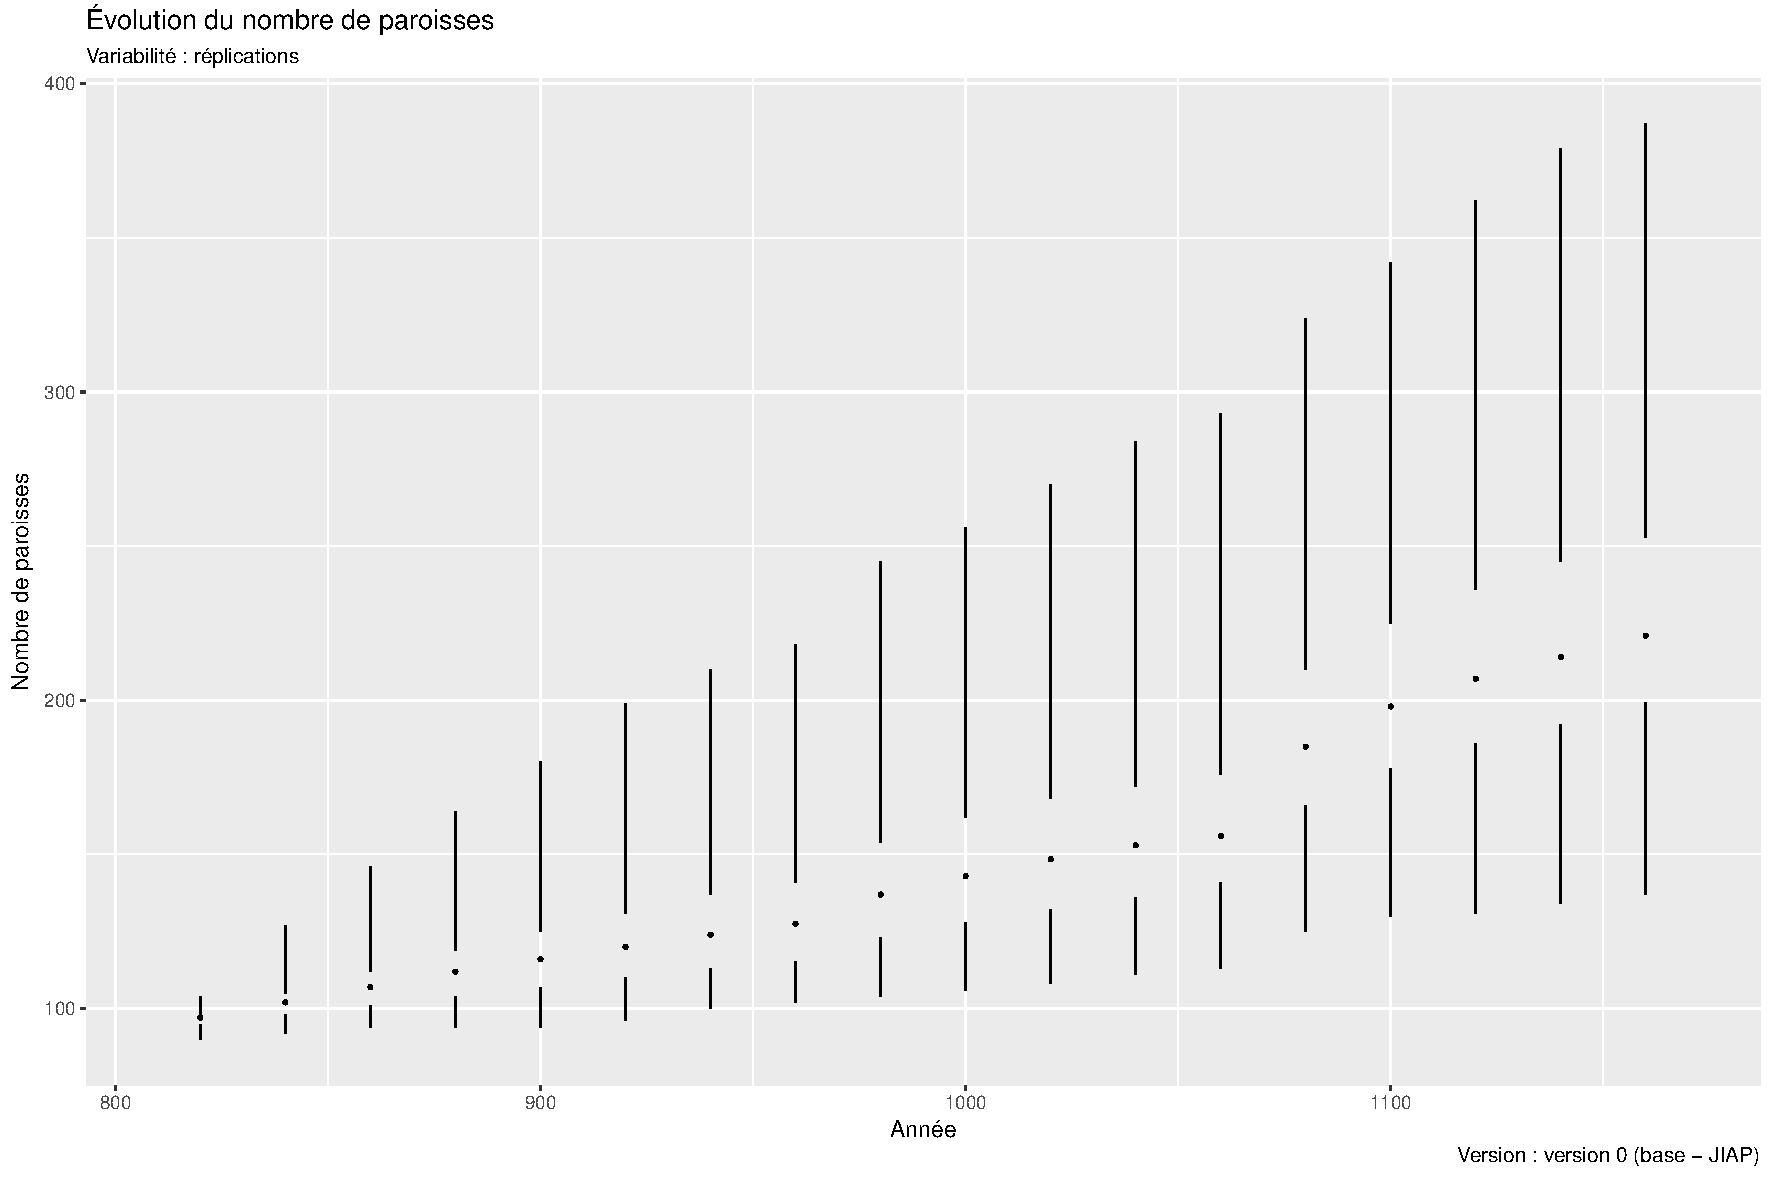
\includegraphics[width=0.75\linewidth]{img/resultats/v0_nombre_paroisses.pdf}
\caption{Évolution du nombre de paroisses}
\label{fig:nb-paroisses-v0}
\end{figure}

\begin{figure}[H]
\captionsetup{width=\linewidth}
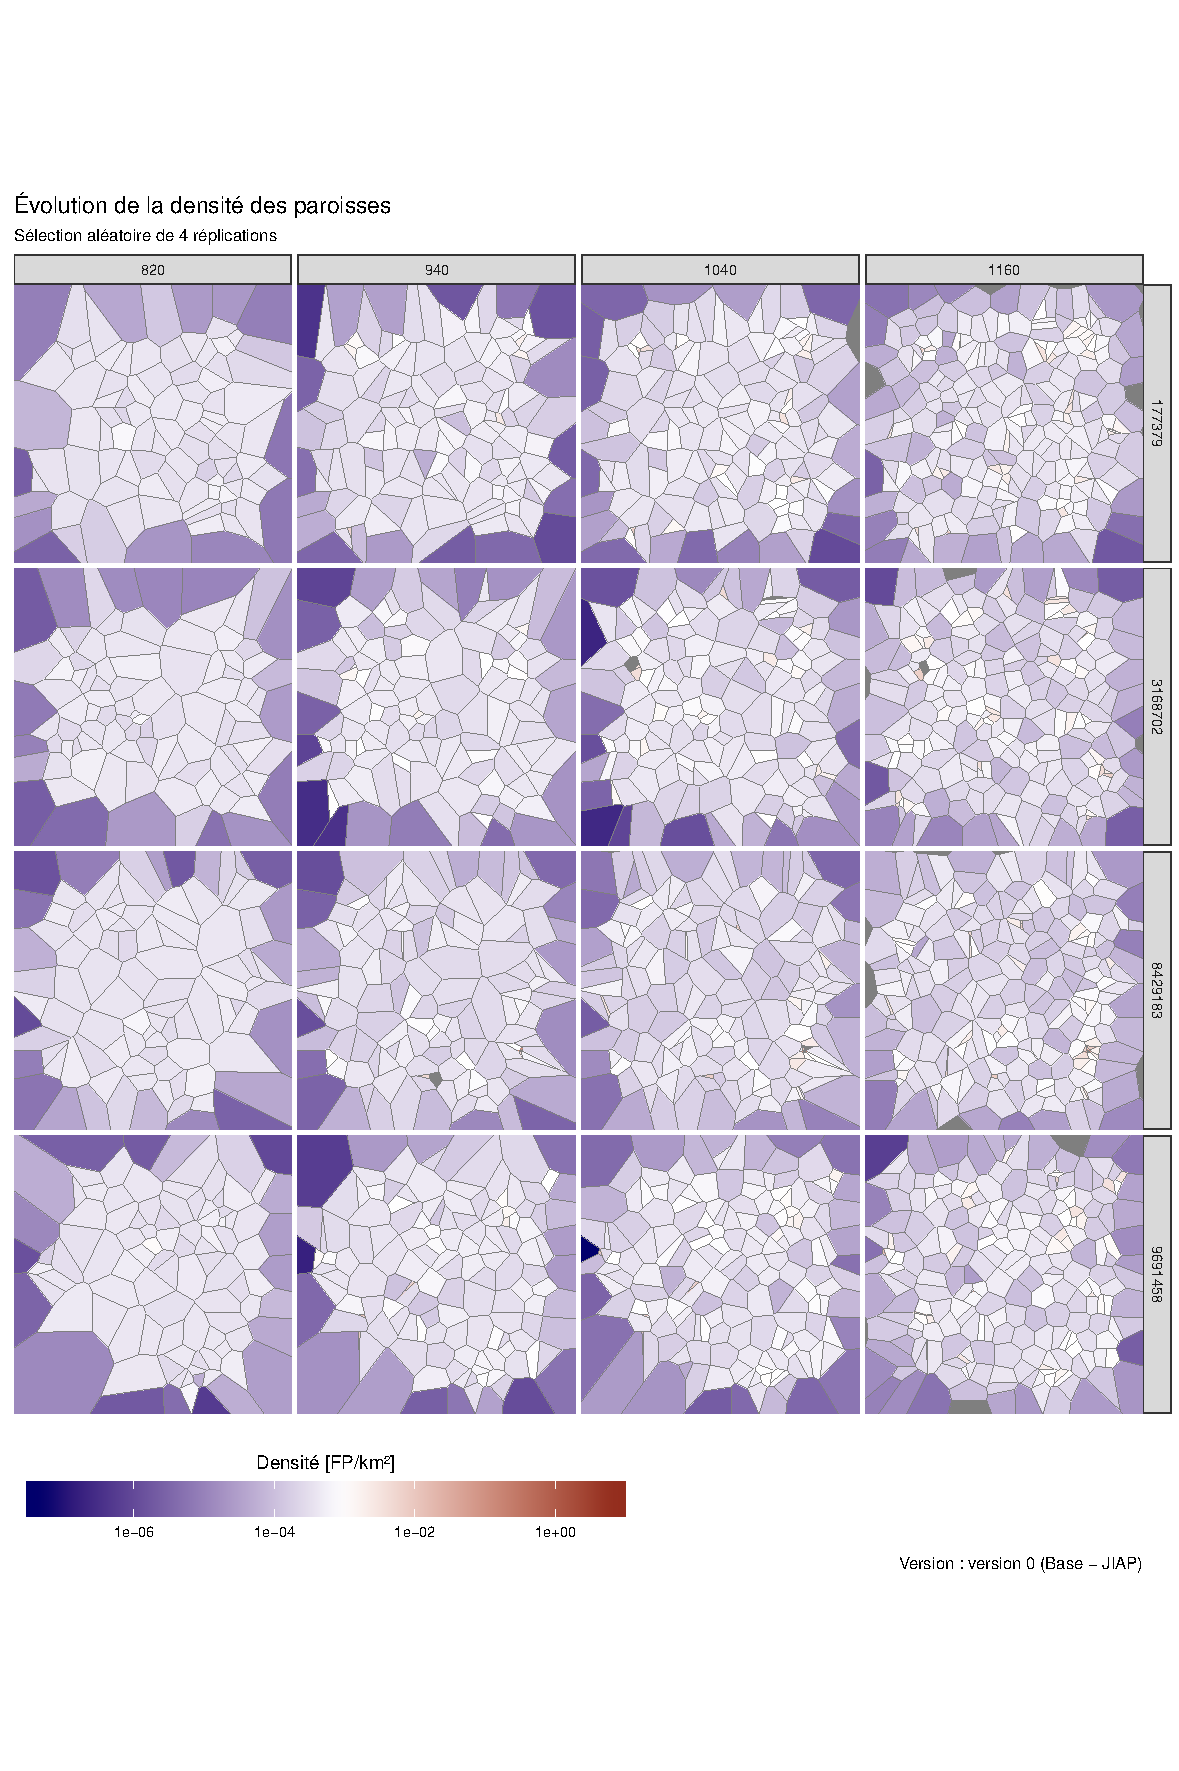
\includegraphics[width=0.8\linewidth]{img/resultats/v0_paroisses_densite.pdf}
\caption{Densité des paroisses}
\label{fig:densite-paroisses-v0}
\end{figure}


\clearpage

\subsubsection{Efficacité et équité de la desserte paroissiale}

On a vu précédemment (\ref{par:hierarchie-paroisses} , \cnameref{par:hierarchie-paroisses}, p. \pageref{par:hierarchie-paroisses}) que les paroisses devaient assurer conjointement une desserte efficace et équitable.
Un indicateur possible pour évaluer l'efficacité du maillage simulé est d'en observer la couverture spatiale.
Par définition, les paroisses couvrent ainsi l'ensemble du territoire simulé.
Pour autant, certaines paroisses peuvent être très étendues, comme vu dans l'indicateur précédent.
On peut toutefois quantifier la dispersion de ces paroisses en analysant leur répartition spatiale, ou plutôt, celle des églises paroissiales qui en constituent le cœur.
Pour cela, on peut faire appel à une méthode d'analyse spatiale assez classique, similaire à la méthode des quadrats, en découpant l'espace en un maillage orthogonal régulier et en comptant le nombre d'églises paroissiales de chacune des mailles.
On a vu que dans SimFeodal, les églises paroissiales sont réparties de manière à la fois dispersée (zones de faible densité) et concentrées (zones denses à proximité des agrégats importants).
Plutôt que de faire un décompte des églises paroissiales et d'en tirer une hiérarchie, un indicateur plus simple est alors de faire un compte des mailles ne contenant pas de paroisse. Ces mailles étant régulières, l'indicateur résultant permettra alors d'appréhender simplement la part de l'espace couvert par des églises paroissiales.
On a choisi ici de discrétiser l'espace modélisé (de dimensions $100\times100$ km) en mailles de $10\times10$ km, pour un total de $100$ mailles de $100$km².
Ces valeurs permettent d'approcher, à grands traits, la configuration théorique qui verrait chacune des 300 églises paroissiales être réparties dans une maille différente\footnote{Il faudrait alors 300 mailles de $\approx$ 6 km de largeur, mais cette valeur ne constitue pas un multiple de 100. De plus, les églises paroissiales étant générées en partie au sein d'agrégats existants pour renforcer la desserte du plus grand nombre, cette valeur est très loin d'être accessible.}.

Selon les mécanismes de SimFeodal, on s'attend à ce que l'indicateur ainsi produit diminue au cours du temps, à mesure que de nouvelles églises paroissiales viennent desservir le territoire, de manière régulière (comme l'évolution du nombre d'églises paroissiales).
Cette diminution devrait toutefois être moins rapide que celle du nombre de paroisses, puisque les églises paroissiales créées au sein des agrégats devraient logiquement ne pas desservir de nouvelles mailles, mais plutôt se situer dans des mailles déjà occupées.

Du point de vue de l'équité de la desserte, on peut recourir à un indicateur plus partiel : il s'agit ici de décrire non pas l'évolution de la desserte des paroisses pour la plupart des foyers paysans, mais plutôt pour ceux d'entre eux qui seraient le plus isolés.
Ainsi, on peut observer l'évolution de la proximité entre les foyers paysans et les églises paroissiales, et ce, pour les paysans les plus éloignés desdites églises paroissiales à chaque pas de temps.
Une augmentation de l'équité devrait ainsi, par exemple pour les 10\% de foyers paysans les moins bien desservis, montrer une diminution de la distance moyenne aux églises paroissiales.

On s'attend ici aussi à voir une augmentation de l'équité, et donc une diminution au cours du temps de cette distance.
Empiriquement, on estime à $5$km la distance maximale à laquelle un foyer paysan se situait d'une église paroissiale en fin de période (\hl{Voir les seuils de distance dans chapitre 2}).
Un paramétrage de SimFeodal sera donc considérée comme satisfaisant, sur ce plan de l'équité de desserte, s'il voit cette distance converger vers le seuil, voire passer en dessous, de $5$km.


\todobox{Il manque un indicateur d'équité. A compléter une fois qu'il sera mis en place. Par exemple :\\
Évolution de la distance des 10\% de FP les plus éloignés d'une/à une église paroissiale ? ==> Sans doute très intéressant, mais pas \og productible\fg{} pour l'instant. De toute façon, à voir les résultats JIAP, il faudra sans doute faire retourner toutes les itérations du modèle avec des sorties semblables à celles de la v8 (4\_4\_A)\\
==> Peut être sous forme de boxplot ou d'histogramme (ridgeplot) ou de moyenne (plus influencée par grandes distances que médiane, donc mieux ici)}

\begin{mdframed}[backgroundcolor=gray!10,footnoteinside=false]

En matière d'efficacité, la version 0 de SimFeodal est assez peu satisfaisante : malgré un nombre d'églises paroissiales trop élevé (voir l'indicateur précédent), la couverture du territoire est assez faible.
En effet, la \cref{fig:couverture-paroisses-v0} montre qu'en fin de simulation, près de $90$\% de mailles restent inoccupées par des églises paroissiales.
La tendance est toutefois à la diminution de ces mailles vides, et cette diminution est assez stable et régulière dans le temps.

Comme dans le cas de l'évolution du nombre de paroisses, la variabilité est ici préoccupante et très insatisfaisante : l'écart interquartile est modéré (environ $15$\%), mais les minimums et maximums présentent un écart énorme (de $95$\% à $55$\%).

\todobox{Pas possible d'analyser les résultats de la version 0 en matière d'équité sans les mesures correspondant. A faire une fois que les graphiques auront été produits.}

\end{mdframed}

\begin{figure}[H]
\captionsetup{width=\linewidth}
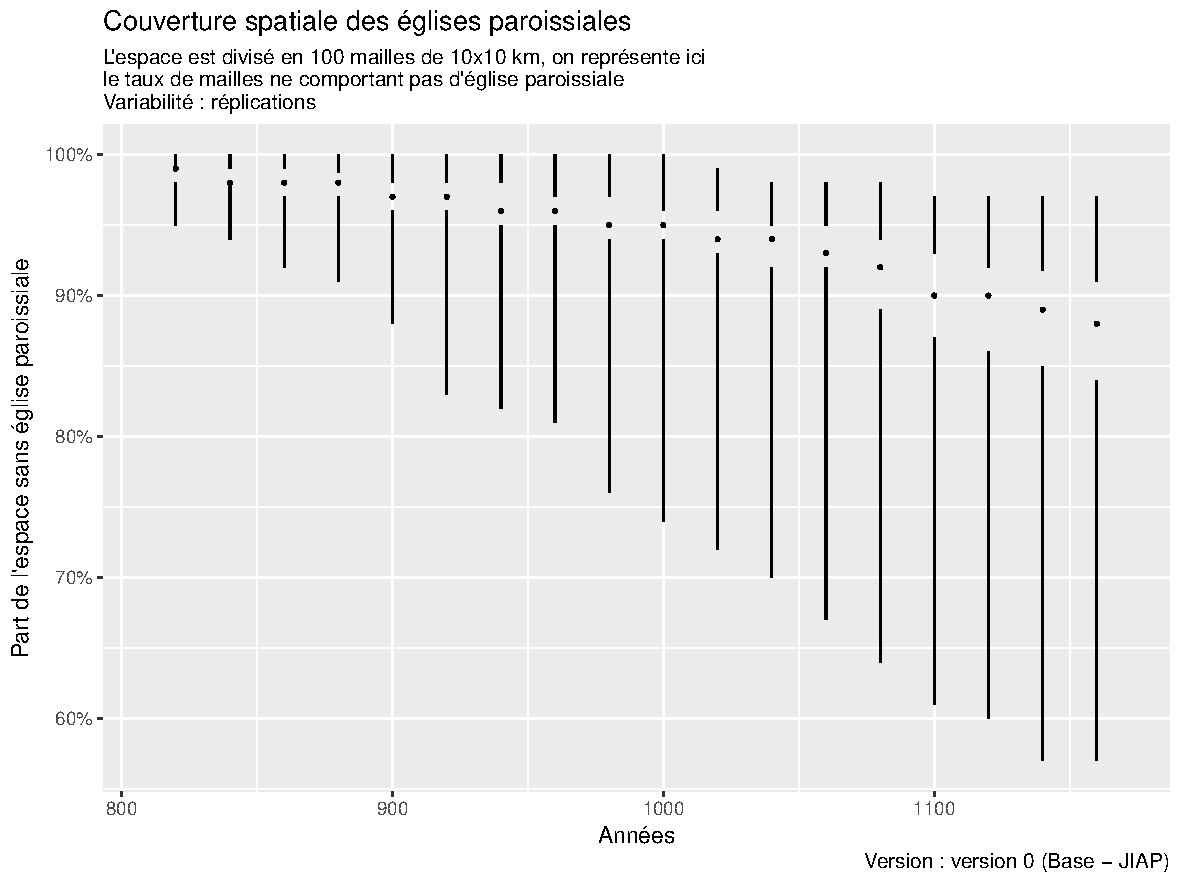
\includegraphics[width=0.9\linewidth]{img/resultats/v0_paroisses_occupation.pdf}
\caption{Évolution de la couverture du territoire par les églises paroissiales.\\
\todobox{Attention, résultats JIAP = pas fiables}
}
\label{fig:couverture-paroisses-v0}
\end{figure}

\printbibliography[title={Références}]
